\newpage
\section{Experimentación}\label{sec:experimentacion}

En esta secci\'on se presentaran los resultados de la experimentaci\'on realizada. Pero previamente es necesario conocer los algoritmos con los cuales se compar\'o nuestra metaheur\'istica.

\begin{enumerate}
\item Scip: Este algoritmo esta realizado con programaci\'on lineal entera y se explica en detalle en la secci\'on \textbf{Programaci\'on Lineal Entera}.
\item Goloso: Este algoritmo es un simple Goloso, es decir, en cada iteracion agrega a la soluci\'on en pad que mas ogip tape.
\item Goloso Maximos Locales: Este algoritmo, en cada iteraci\'on busca el pad de mayor ogip (al igual que el goloso), pero como esto esta ligado a la discretizaci\'on, a este pad se lo mueve tratando de ubicarlo en alg\'un lugar cercano donde tenga mayor ogip, es decir, no importa al 100\% la discretizaci\'on, dado que se consigue un pad centrado en la discretizaci\'on (este pad es el pad con mayor ogip de todos los pads centrados en la discretizaci\'on) y luego busco un m\'aximo local en los alrededores y una vez encontrado lo agrega a la soluci\'on.

Para esto, se utiliza un par\'ametro \textbf{Paso Movimiento Pad} que indica el paso que se tiene en cuenta a la hora de mover el pad buscando el m\'aximo local. 

Una vez que no tengo m\'as pads disponibles puede haber pasado que al mover los pads, no tenga m\'as pads disponibles de los centrados en la discretizaci\'on, pero si existen huecos donde entran otros, por lo tanto, se \textbf{re-discretiza} el \'area no tapada hasta el momento, se hace una discretizaci\'on m\'as fina, y para esto se usa el p\'arametro \textbf{Paso mejora Discretizaci\'on} que indica en cuanto se achica la discretizaci\'on. Luego se vuelve a calcular los posibles pads para esta nueva discretizaci\'on. Notar que solo se discretiza mas fino los sectores no tapados por los pads provenientes de la discretizacion m\'as gruesa.

Por ejemplo, en las siguientes figuras podemos ver como en la primera el paso de la discretizaci\'on es m\'as grueso que en la segunda (marcado en rojo). Y tambi\'en podemos ver como la discretizaci\'on en la segunda solo se hace en los luegares no tapados. Notar que la discretizaci\'on esta marcada con puntos en la regi\'on.

\begin{center}
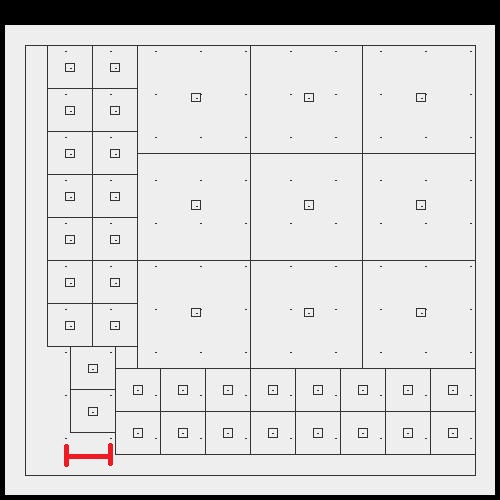
\includegraphics[width=0.4\textwidth]{imagenes/iter40}
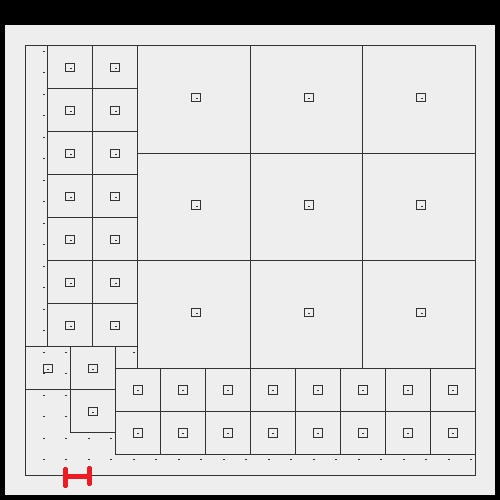
\includegraphics[width=0.4\textwidth]{imagenes/iter45}
\end{center}

\end{enumerate}


Antes de continuar se explican que son cada item de los resultados obtenidos:

\begin{enumerate}
\item Tiempo: Tiempo que se tard\'o en encontrar \textbf{la mejor soluci\'on}.
\item Cant. Pads: Cantidad de pads que tiene la soluci\'on.
\item Area (\%): Porcentaje de \'area que se consigu\'o tapar con los pads de la soluci\'on.
\item Ogip: El ogip que se consigui\'o tapar con los pads de la soluci\'on.
\item Area Superpuesta (del total cubierto) (\%): Porcentaje de \'area superpuesta por los pads de la soluci\'on. (Porque en scip se pisan).
\item Cant. Ar. Cubierta: Valor del area cubierta.
\item Cant. Ar. Superpuesta: Valor de area superpuesta.
\item Ar. Region: Total de la regi\'on de la instancia.
\item Iter. Sol.: N\'umero de iteraci\'on que se consigue la mejor soluci\'on.

\end{enumerate}

				

Lo primero que se hizo fue un an\'alisis de la variaci\'on de los par\'ametros. Entonces analizando los resultados en la secci\'on \textbf{anexo} se concluy\'o que los par\'ametros CITF (Cantidad Intentos de Tapar una Feromona), FCF (Factor Cambio Feromona), IMPSR (Intentos Meter Pad soluci\'on Random) se van a dejar fijos. Por otro lado, se decidi\'o hacer que CSRI = CSNRPI dadol que no importa que iteraci\'on sea, siempre dajamos seteada la cantidad de soluciones en un mismo valor. 

Entonces los par\'ametros que nos quedaron para variar son CSRI (Cantidad soluciones Random Iniciales = Cantidad soluciones No Random Por Iteraci\'on) , CI (Cantidad de Iteraciones), MCBS (Modo Chequeo Buena soluci\'on), DF (Discretizaci\'on Feromona)

A la hora de analizar el tiempo vemos que el par\'ametro MCBS no influye, por lo tanto no lo tenemos en cuenta para esta experiemtanci\'on (Nota, se puede ver que el tiempo cambia levemente si se cambia el MCBC, pero nada significativo). 

Lo primero que se analiz\'o fue el tiempo de ejecuci\'on si se varia la cantidad de soluciones por iteraci\'on, y para eso observemos la siguiente tabla:

\begin{center}
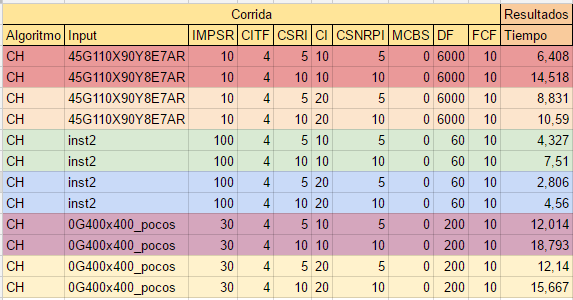
\includegraphics[width=0.6\textwidth]{imagenes/tabla1}
\end{center}

En esta tabla podemos observar 6 subconjuntos de resultados agrupados entre s\'i, donde para cada subconjunto, todos los par\'ametros se mantienen igual excepto la cantidad de iteraciones que varia entre y 5 y 10 (par\'ametros CSRI y CSNRPI). Se puede ver que en todos los casos el tiempo aumenta considerablemente al aumentar la cantidad de soluciones por iteraci\'on, en particular, se puede ver en el primer caso (filas rojas) que al duplicar la cantidad de soluciones por iteraci\'on, el tiempo aumenta a mas del doble (pasa de 6 a 14 segundos).

Observemos que pasa con el algoritmo de colonia de hormigas versi\'on 2:

\begin{center}
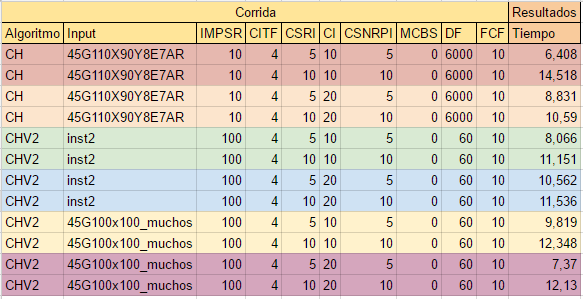
\includegraphics[width=0.6\textwidth]{imagenes/tabla2}
\end{center}

En esta tabla podemos observar lo mismo que en el caso anterior, es decir, al aumentar la cantidad de soluciones el tiempo aumenta. Pero vale destacar que en instancias como \textbf{inst2}, que es una instancia pequeña, el tiempo aumenta poco.

Todos estos resultados tienen sentido, dado que, sin importar la versi\'on que se utilice del algoritmo, para cada soluci\'on encontrada tenemos que aumentar la feromona, y la l\'ogica de actualizaci\'on de feromona demora bastante, mas alla del tiempo que demora en conseguir la propia soluci\'on. 

A continuaci\'on vamos a analizar que pasa con el tiempo al variar el otro par\'ametro, que es el CI (Cantidad de Iteraciones). 

\begin{center}
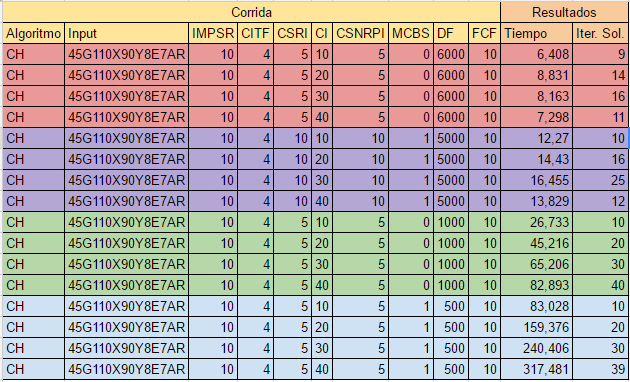
\includegraphics[width=0.6\textwidth]{imagenes/tabla3}
\end{center}

En esta tabla se pueden ver 4 subconjunto de corridas (rojo, violeta, verde y azul). Veamos a continuaci\'on, como se refleja esto en una gr\'afico de lineas.

\begin{center}
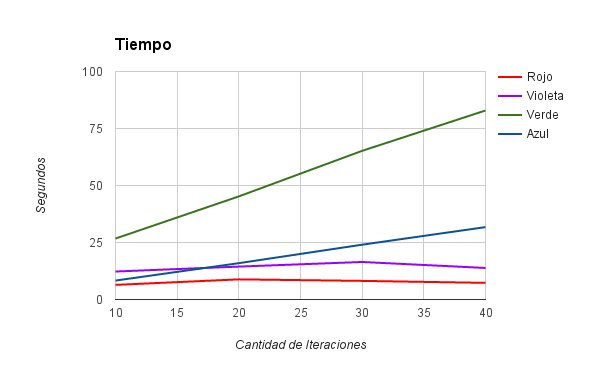
\includegraphics[width=0.6\textwidth]{imagenes/grafico1}
\end{center}

Podemos ver tanto en la tabla como en el gr\'afico, que a medida que aumentamos la cantidad de iteraciones, aumenta el tiempo, excepto en el caso del rojo y violeta. Esto es a causa del que el tiempo, es el tiempo hasta encontrar la mejor soluci\'on y si miramos con detalle la columna Iter. Sol., vamos a observar que en los dos casos que el tiempo disminuye es porque la mejor soluci\'on se encontro antes que los casos anteriores. Este resultado es un resultado correcto, dado que puede pasar que la soluci\'on se encuentre antes ya que cada soluci\'on es distinta de las otras y adem\'as se comienza con soluciones randoms. 
Por lo tanto vemos que no siempre aumentar la canitad de iteraciones es bueno para mejorar el tiempo ya que encontramos casos donde aumentamos las iteraciones y se tard\'o m\'as, pero por otro lado encontramos casos donde aumentamos las iteraciones y se tardo\'o menos y vale aclarar que existen casos donde se aument\'o la cantidad de iteraciones y la soluci\'on se encontr\'o en un n\'umero de iteraci\'on que era posible encontrar en casos anteriores.

Nota: en el gr\'afico los valores muy elevados se normalizaron (se lo dividi\'o por 10) para que el gr\'afico quede prolijo.

\newpage

Veamos ahora que pasa usando colonia de hormigas versi\'on 2:

\begin{center}
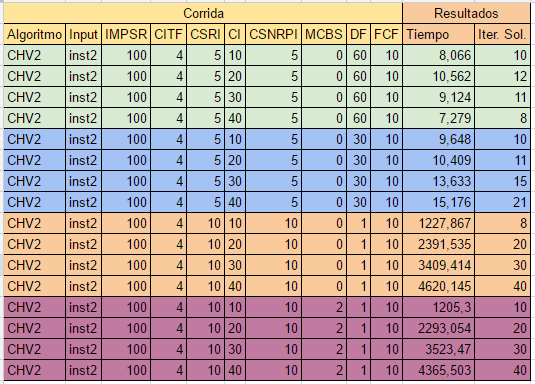
\includegraphics[width=0.6\textwidth]{imagenes/tabla4}
\end{center}

En esta tabla se pueden ver 4 subconjuntos de corridas (verde, azul, naranja y violeta). Veamos a continuaci\'on, como se refleja esto en una gr\'afico de lineas.

\begin{center}
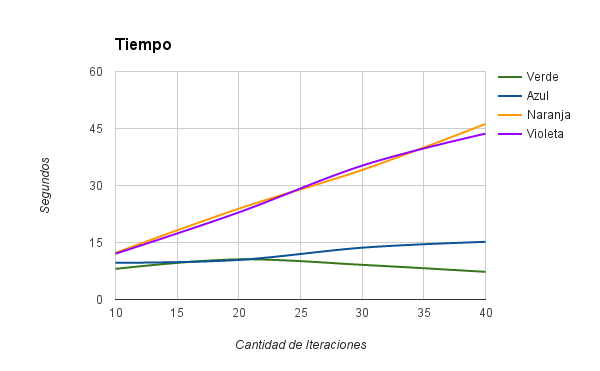
\includegraphics[width=0.6\textwidth]{imagenes/grafico2}
\end{center}

Se puede ver, al igual que en la versi\'on 1, que la versi\'on 2 se comparta igual, es decir al aumentar la cantidad de iteraciones aumenta el tiempo, pero en algunos casos el tiempo disminuye debido a que la soluci\'on se encontr\'o en una interaci\'on mucho antes.

A continuaci\'on vamos a analizar que sucede con el tiempo al variar, para distintas instancias, la discretizaci\'on de la feromona. 

\begin{center}
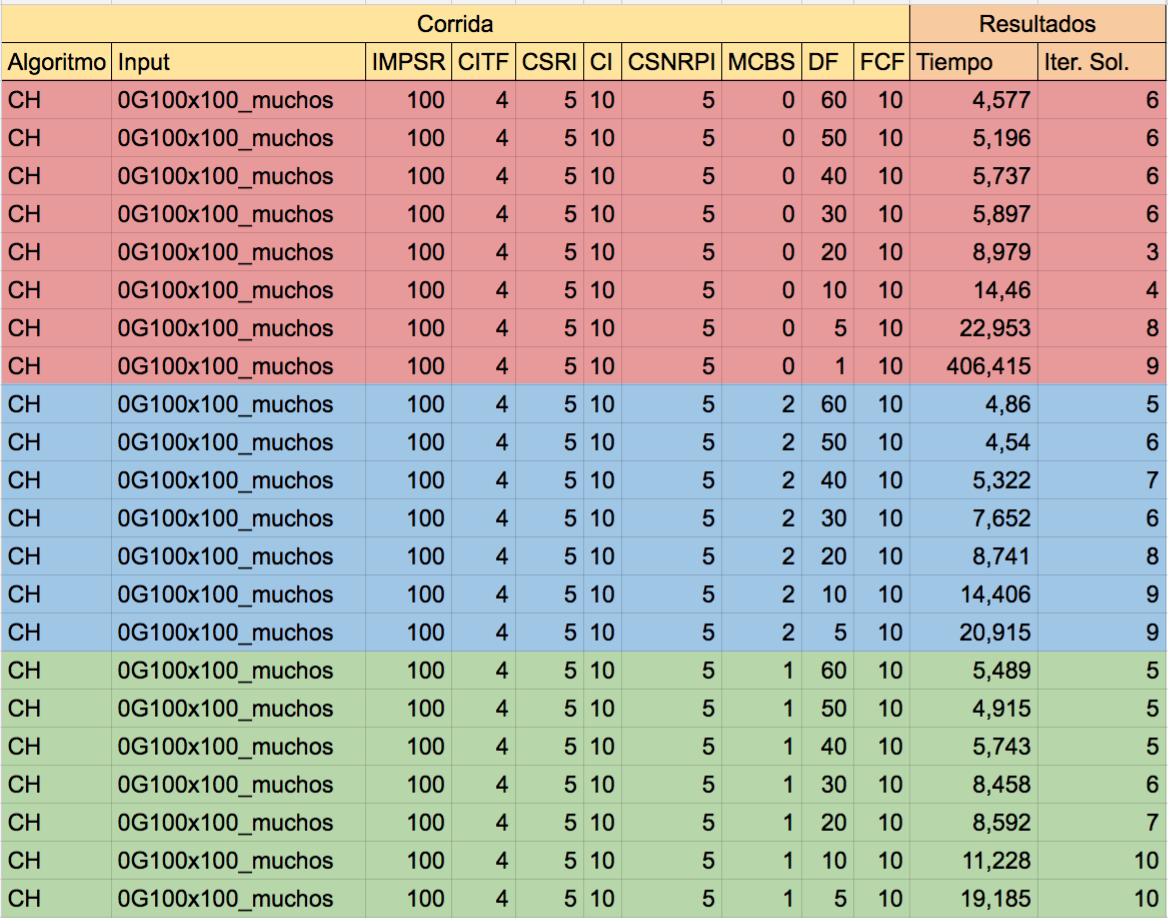
\includegraphics[width=0.6\textwidth]{imagenes/tabla5}
\end{center}



\begin{center}
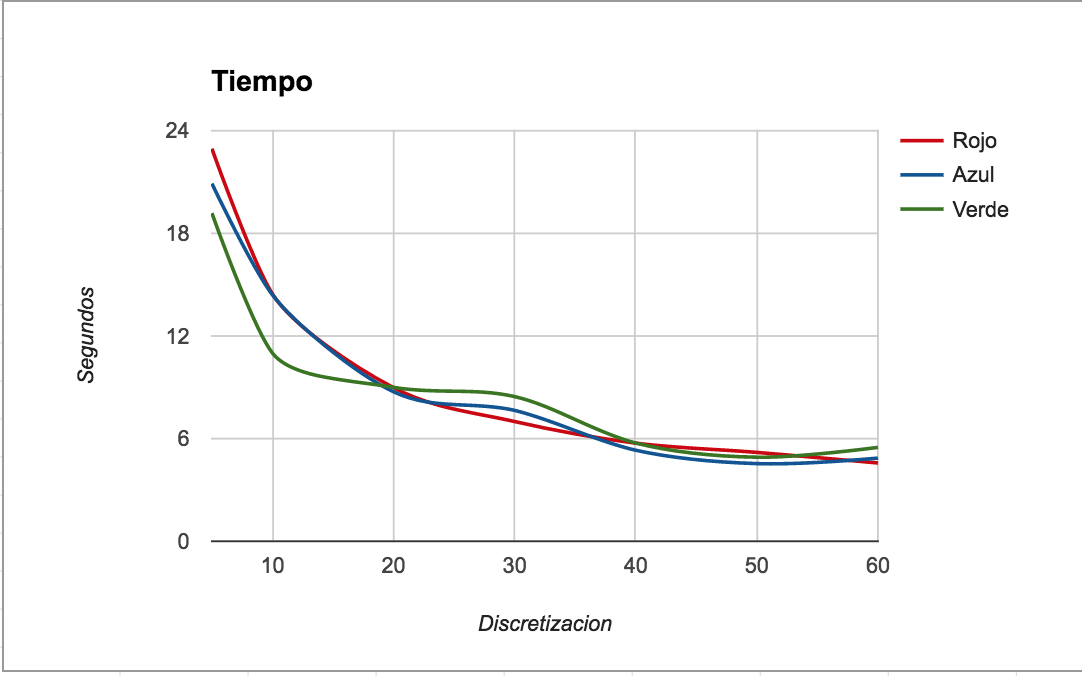
\includegraphics[width=0.6\textwidth]{imagenes/grafico3}
\end{center}




Se puede ver claramente en estos dos gr\'aficos como al disminuir la discretizaci\'on (es decir, discretizar mas fino), el tiempo aumenta considerablemente. Esto es l\'ogico, dado que la matriz de feromonas es mucho m\'as grande al disminuir el valor de la discretizaci\'on y por cada soluci\'on tenemos que iterarla por completo para actualizarlo.
Notar tambi\'en que no importa si la mejor soluci\'on se encontr\'o antes o despu\'es (si se encontr\'o de forma temprana o no) dado que la mayor cantidad de tiempo se pierde actualizando la feromona y aunque la mejor soluci\'on la encuentre r\'apido vamos a tener que actualizar hasta la \'ultima soluci\'on. Se puede ver un caso en las filas rojas, donde una soluci\'on se encontr\'o en la iteraci\'on 6 tardando 6 seg aproximandamete y en la fila siguiente se encuentra la soluci\'on en la iteraci\'on 3 pero se tarda 9 segundos aproximadamente.

\newpage

Veamos un ejemplo con otra instancia,

\begin{center}
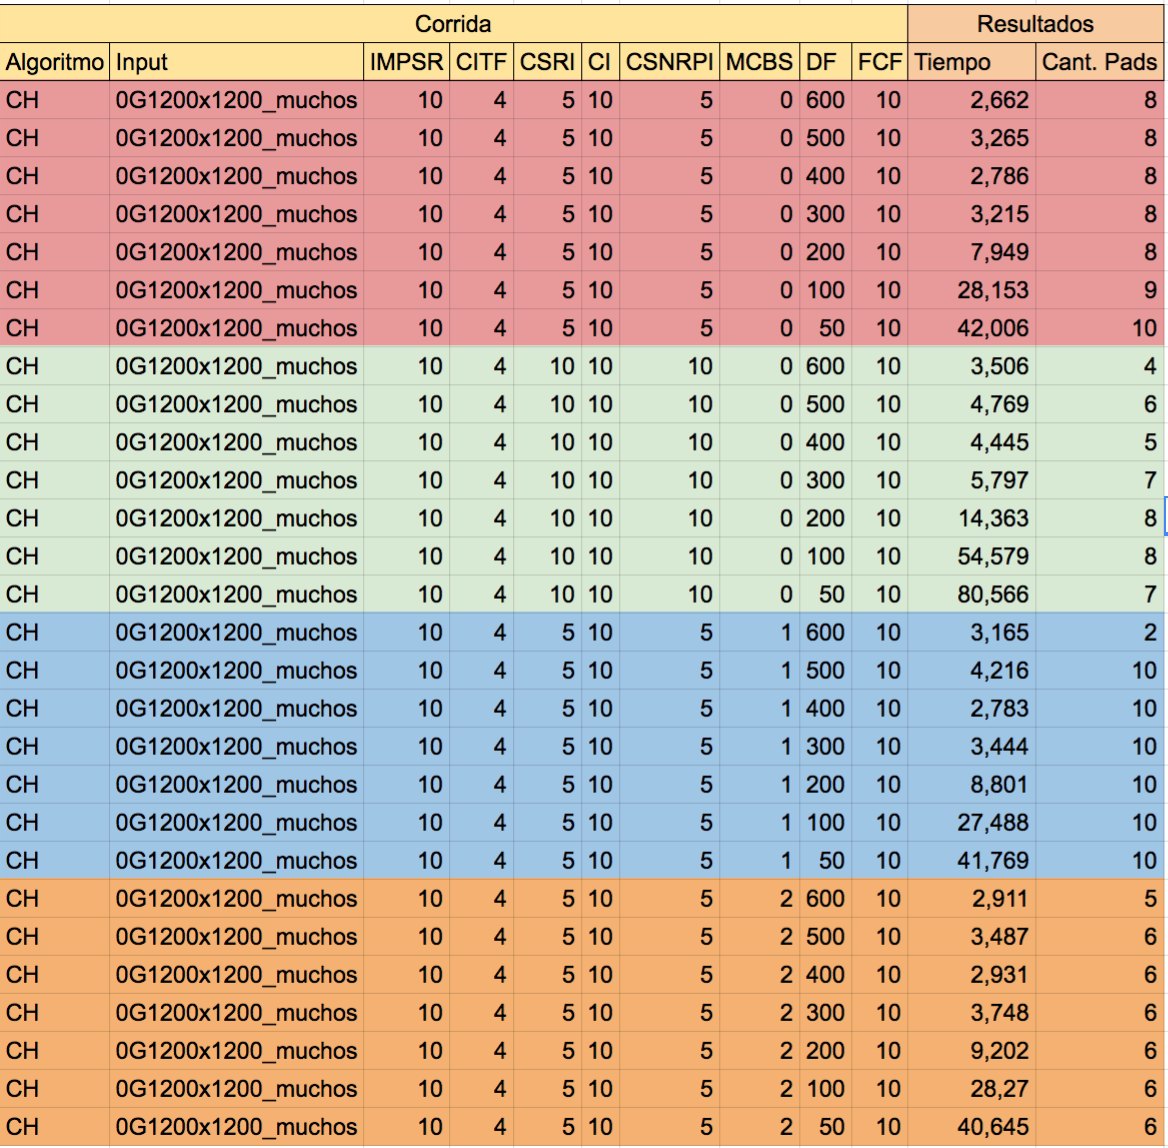
\includegraphics[width=0.6\textwidth]{imagenes/tabla6}
\end{center}


\begin{center}
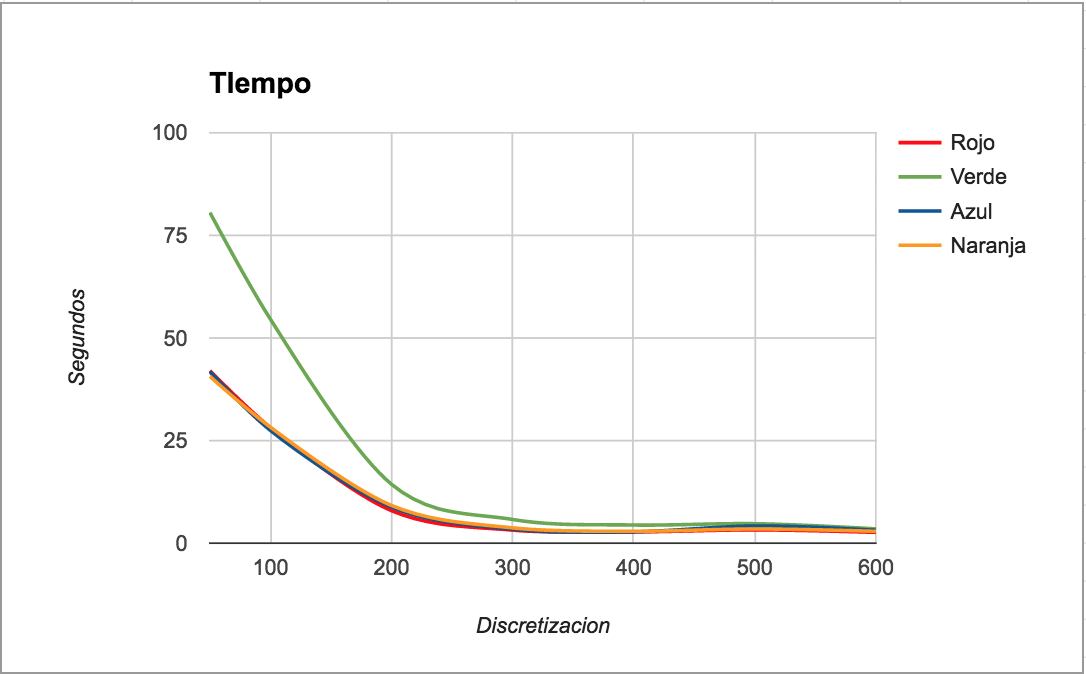
\includegraphics[width=0.6\textwidth]{imagenes/grafico6}
\end{center}


En este ejemplo se puede notar lo mismo que en el anterior, vemos en el gr\'afico de lineas como es claro que a medida que se discretiza m\'as fino (se achica el valor) la discretizaci\'on tarda mucho m\'as. 

A continuaci\'on, vamos a comparar los resultados de tiempos entre todas las intancias y todos los algoritmos, para eso agarramos la ejecuci\'on que mejor ogip consigui\'o para una instancia y las ponemos en la siguiente tabla:

\begin{center}
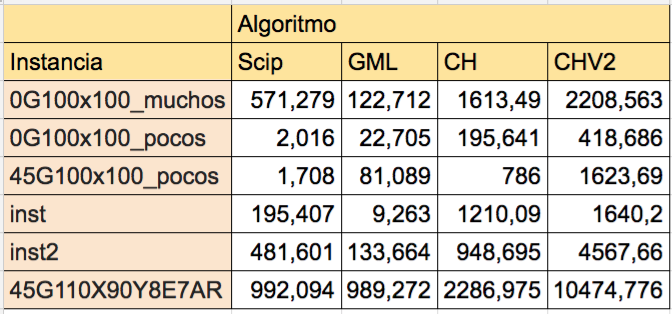
\includegraphics[width=0.5\textwidth]{imagenes/tabla10}
\end{center}

\begin{center}
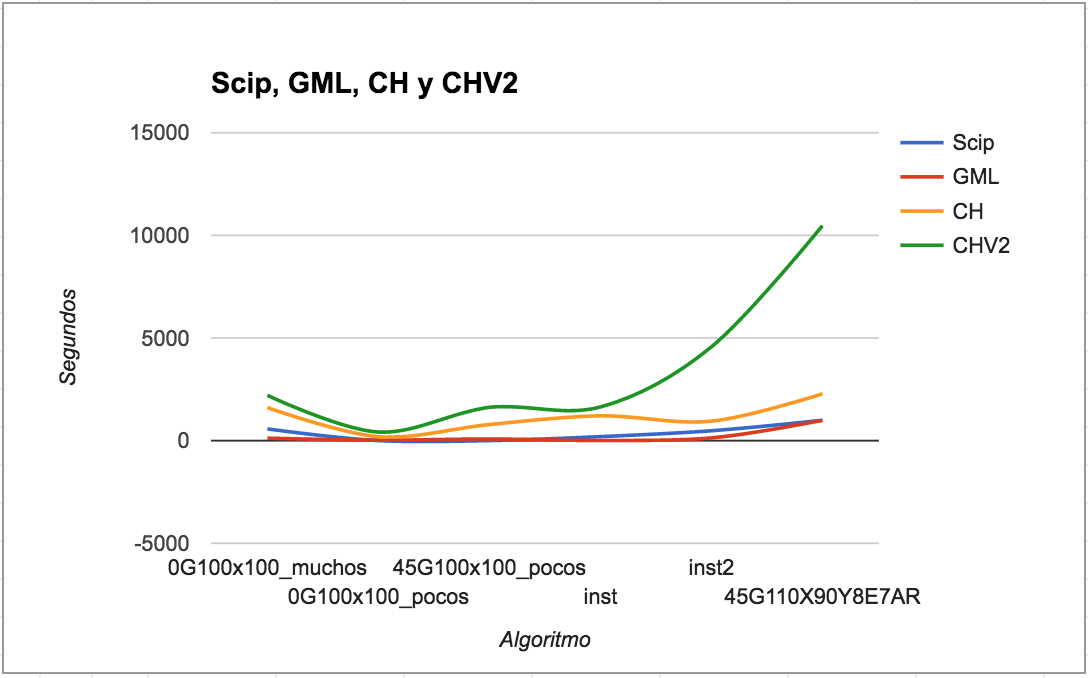
\includegraphics[width=0.6\textwidth]{imagenes/grafico10}
\end{center}


Se puede ver claramente como el algoritmo de Colonia de Hormigas tarda mucho mas que el resto, esto es claro dado que en este algoritmo se recorre toda la discretizaci\'on en cada soluci\'on para actualizar la feromona (Esto es un detalle de implementacion que se podr\'ia mejorar en trabajos futuros). 
Tambi\'en se puede notar como la versi\'on 2 del algortimo de Colonia de Hormigas tarda m\'as que la version 1, lo cual tambi\'en es l\'ogico, dado que en este algoritmo tenemos mas cantidad de feromonas y entonces tenemos que recorrer m\'as (una feromona por semilla).

Pero es importante notar algunos resultados obtenidos en las siguientes tablas:

\begin{center}
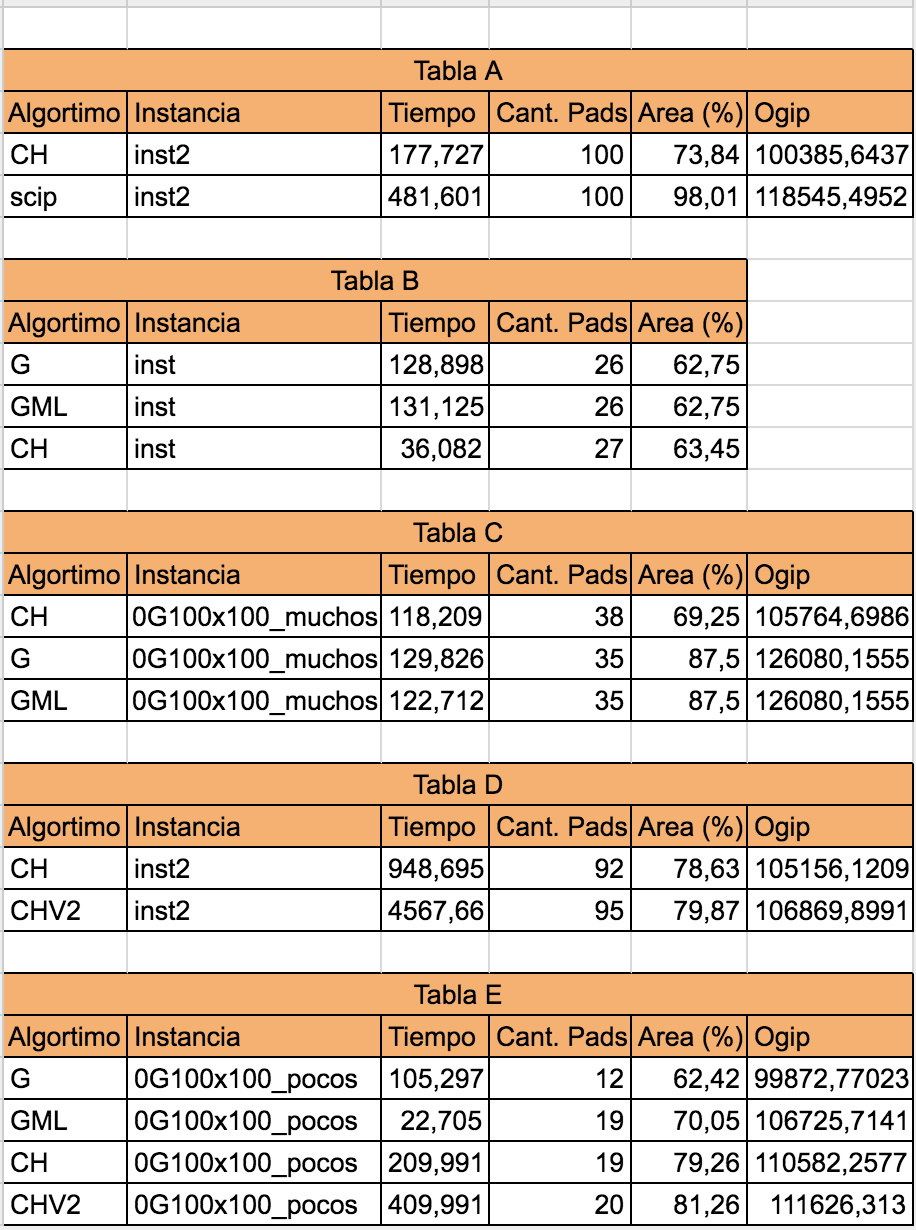
\includegraphics[width=0.5\textwidth]{imagenes/tabla11}
\end{center}

En la Tabla A se puede ver que, aunque el algoritmo de Colonia de Hormigas no consiga tener un valor de ogip tan bueno como Scrip, este tarda mas de la mitad del tiempo.

En la Tabla B se puede ver que el algoritmo de Colonia de Hormigas tarda mucho menos, y consigue un ogip mejor que el del Goloso y el del Goloso Maximos Locales.

En la Tabla C se puede ver que el algortimo de Colonia de Hormigas no es tan bueno como G y GML, pero tarda menos tiempo.

En la Tabla D se puede ver que la Version 2 de Colonia de Hormigas tarda mucho mas pero logramosobtener un ogip mejor.

En la Tabla E se puede ver que el algoritmo de Colonia de Hormigas tarda mucho mas pero consigue un valor mucho mejor y que la version 2 tarda mas y consigue una mejor soluci\'on.

A continuaci\'on haremos un an\'alisis del Ogip, variando los par\'ametros CSRI (Cantidad soluciones Random Iniciales = Cantidad soluciones No Random Por Iteracion) , CI (Cantidad de Iteraciones), MCBS (Modo Chequeo Buena soluci\'on), DF (Discretizaci\'on Feromona)

Variemos el CSRI y CSNRI, es decir la cantidad de soluciones por iteraci\'on:

\begin{center}
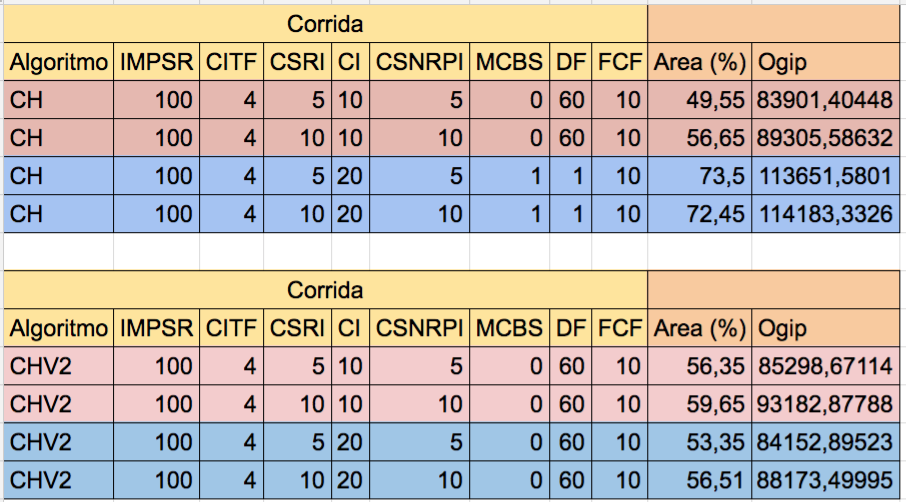
\includegraphics[width=0.6\textwidth]{imagenes/tabla14}
\end{center}

Podemos ver en las tablas que si aumentamos la cantidad de soluciones por iteraci\'on, el ogip conseguido es mayor. Adem\'as podemos ver como la versi\'on 2 obtiene mejores resultados que la versi\'on 1.

Analicemos que pasa al variar la cantidad de iteraciones (CI)

\begin{center}
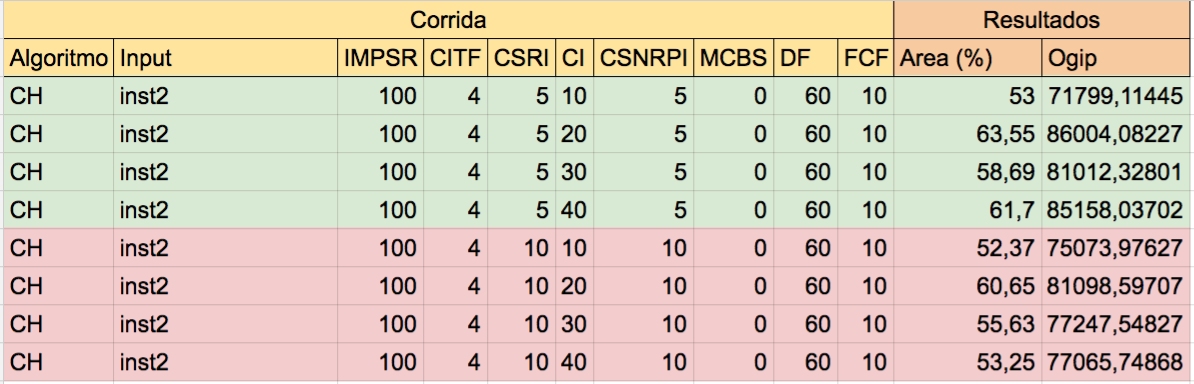
\includegraphics[width=0.6\textwidth]{imagenes/tabla15}
\end{center}

\begin{center}
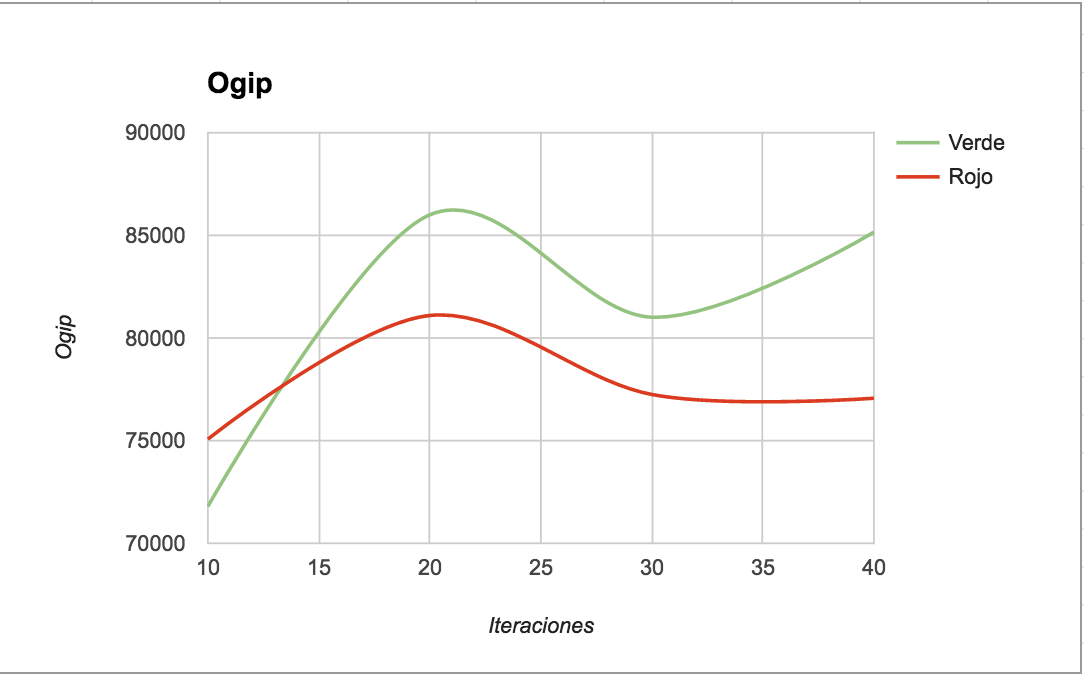
\includegraphics[width=0.6\textwidth]{imagenes/grafico15}
\end{center}

Podemos ver que no siempre a medida que se aumentan las iteraciones el ogip aumenta. Pero es importante aclarar que la discretizaci\'on (60) es un valor muy grande para esta instancia. 

\newpage
Veamos un caso donde discretizamos mas fino.

\begin{center}
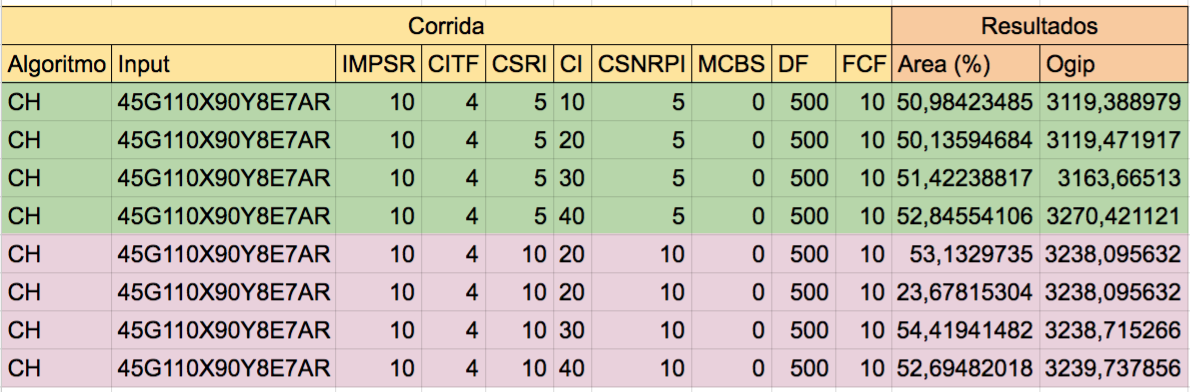
\includegraphics[width=0.6\textwidth]{imagenes/tabla18}
\end{center}

\begin{center}
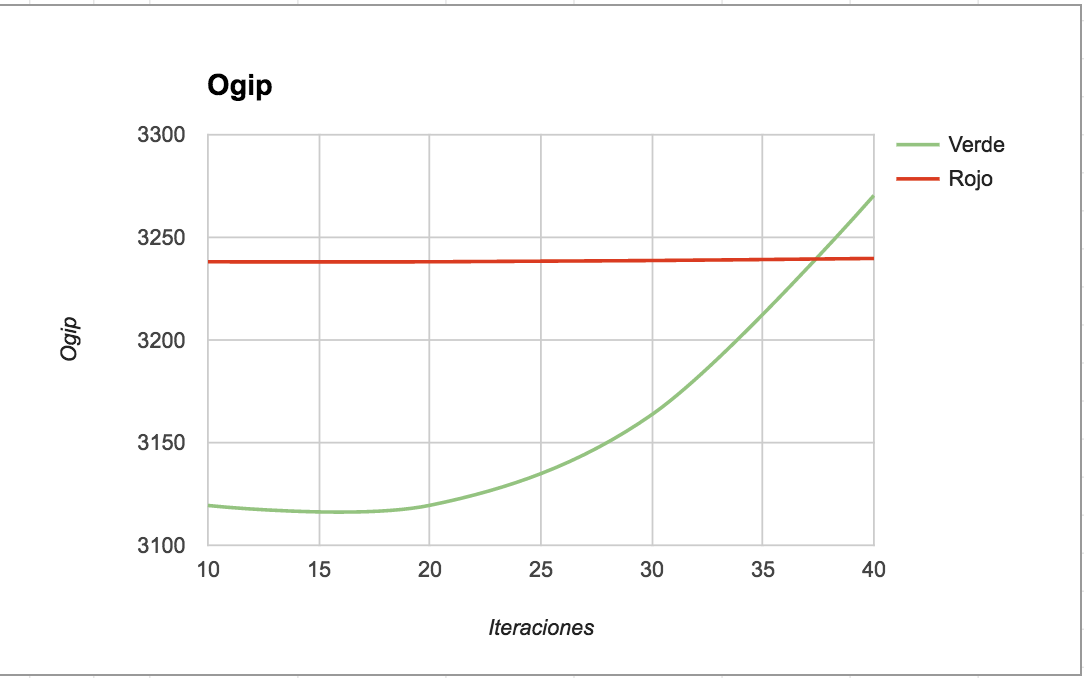
\includegraphics[width=0.6\textwidth]{imagenes/grafico18}
\end{center}

Aca podemos ver que el ogip se mantiene un poco mas estable. No se incluyen gr\'aficos de la version 2 de colonias de hormigas pero los resultados obtenidos se comportan igual (ver secci\'on anexo).

Analicemos a continuaci\'on que pasa al cambiar el MCBS (Modo Chequeo Buena soluci\'on):

\begin{center}
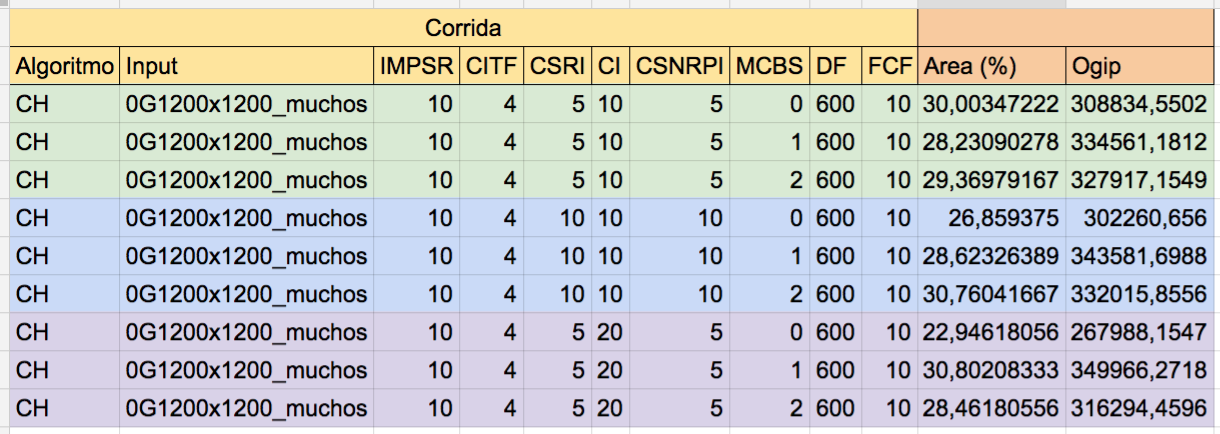
\includegraphics[width=0.6\textwidth]{imagenes/tabla19}
\end{center}


Podemos ver claramente que con el caso 1 es mejor que el resto, seguido del 2 y terminando con el 0. Vease secci\'on algortimo propuesto para ver que signfican cada valor de MCBS.


Miremos el siguiente ejemplo con la version 2 del algoritmo:

\begin{center}
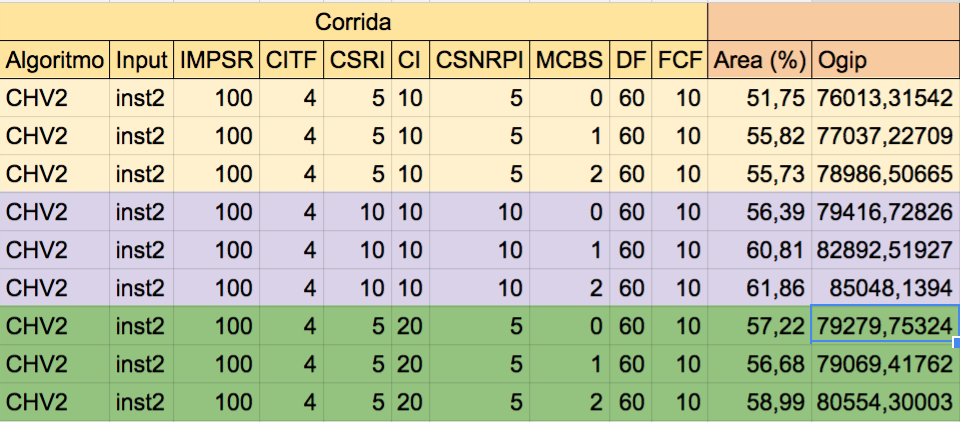
\includegraphics[width=0.5\textwidth]{imagenes/tabla20}
\end{center}

En un principio parace que el modo 2 es mejor que el resto, segudo del 1 y luego del 0, pero en el caso verde podemos ver que el modo 0 es mejor que el modo 1.

\newpage

Analicemos que pasa variando la discretizaci\'on y viendo el ogip:


\begin{center}
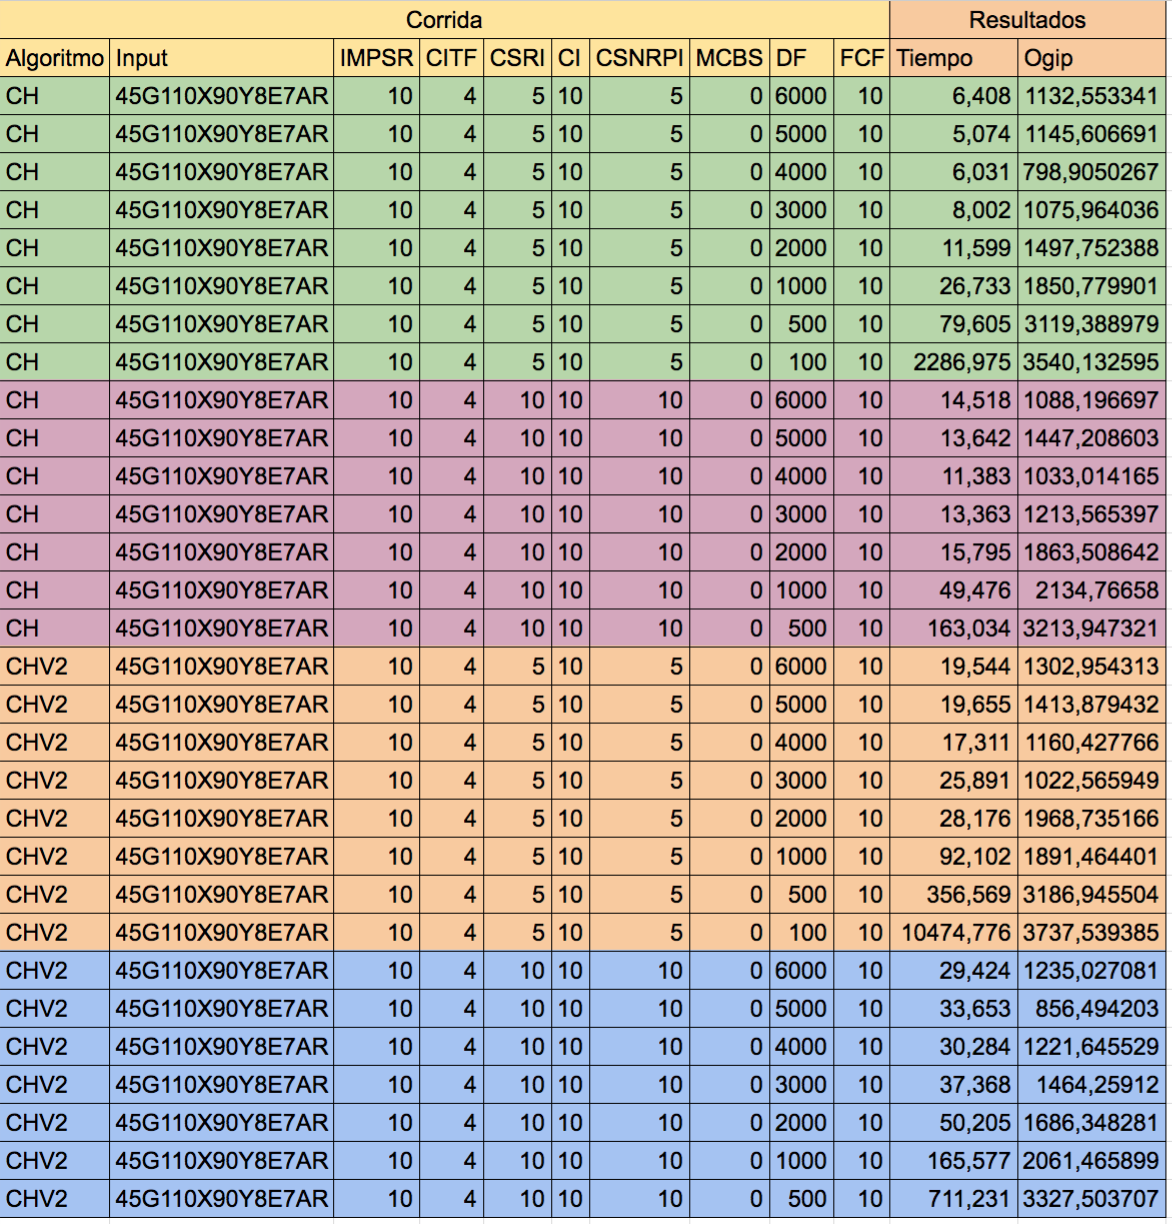
\includegraphics[width=0.7\textwidth]{imagenes/tabla21}
\end{center}

\begin{center}
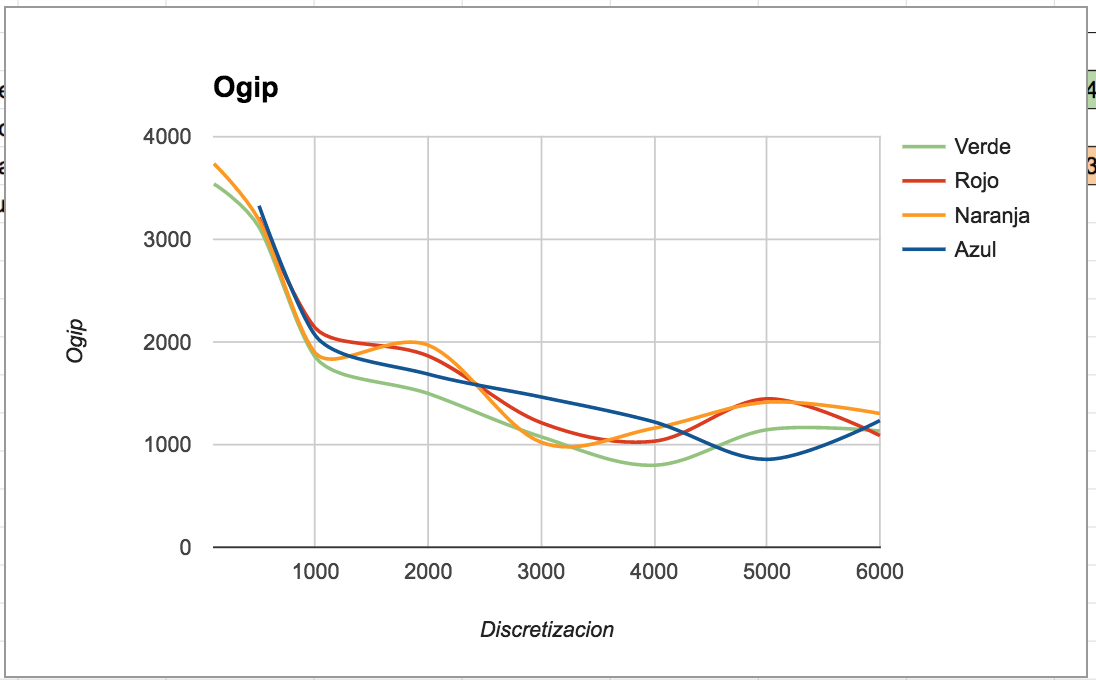
\includegraphics[width=0.6\textwidth]{imagenes/grafico21}
\end{center}

En esta tabla se puede observar una corrida con ambas versiones del algoritmo de colonia de hormigas, y en ambos casos se los separa por subconjuntos (de colores) para poder ver que pasa al variar la discretizaci\'on.

En todos los casos se observa como al discretizar mas fino, el valor del ogip aumenta, excepto en el naranja, que disminuye levemente en un caso (caso an\'omalo). Esto es l\'ogico, dado que al tener la feromona mas discretizada, la cantidad de puntos de la feromona es mayor y por lo tanto puede encontrar el punto mas caliente con mejor precisi\'on. Como fue explicado con anterioridad, al tener mayor discretizaci\'on, la cantidad de pads posibles aumenta y la feromona tambi\'en, esto hace que el problema sea mas lento computacionalmente (como vimos en gr\'aficos anteriores). 

Pero como era de esperarce el ogip mejora al discretizar mas fino.

\newpage

Comparemos los ogip de todos los algoritmos, para esto tomamos el mejor ogip de cada instancia y cada algoritmo y armamos la siguiente tabla:

\begin{center}
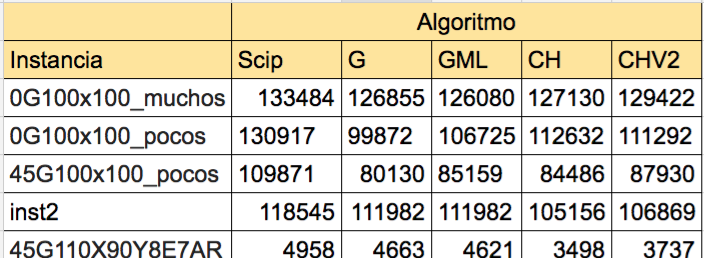
\includegraphics[width=0.5\textwidth]{imagenes/tabla22}
\end{center}

\begin{center}
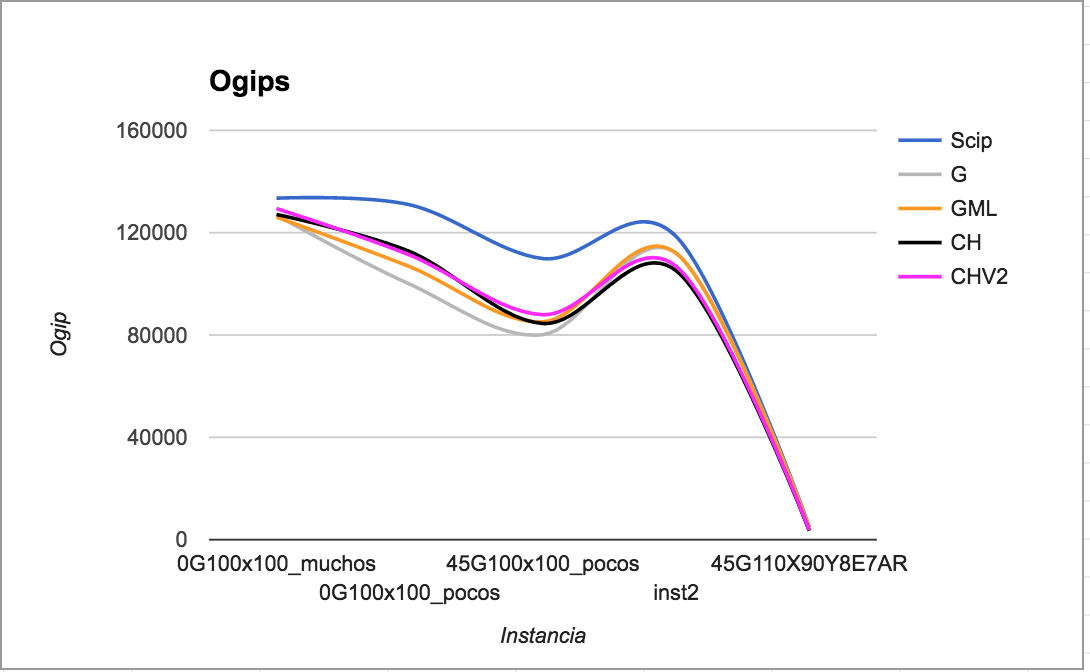
\includegraphics[width=0.6\textwidth]{imagenes/grafico22}
\end{center}

Se puede ver claramente como el algoritmo de Colonia de Hormigas (versi\'on 1, color negro) nunca le gana al Scip, pero esto es l\'ogico, dado que el Scip es un algoritmo exacto y no solo eso, sino que tambi\'en acepta superposiciones, lo cual, los demas algoritmos no hacen superposiciones de pads (ver anexo para saber los porcentajes de superposici\'on).

Por otro lado se ve como Colonia de Hormigas le gana en muchos casos al Goloso com\'un y en algunos puntos es mejor que el Goloso de Maximos Locales.

Tambien vemos que el Colonia de Hormigas Version 2, casi siempre es mejor que el algoritmo en la version 1.


\newpage

Hagamos un analisis de la feromona:

A continuaci\'on podemos ver unos gr\'aficos de la feromona de la versi\'on 1, y vemos como a medida que avanzan las iteraciones la feromona va tomando una forma de picos (asi es como es el ogip en la region). De modo que la feromona m\'as caliente es la correspiente al punto en el plano donde esta el ogip de mayor valor.

Nota: La instancia corrida tiene el ogip creciente para un vertice (como se ve en la feromona) y tiene 3 picos, 2 picos en la parte de mayor ogip y un pico en la parte de menor ogip. Por lo tanto podemos decir que la feromona tiende a asemejarse a la funci\'on de ogip.


\begin{center}
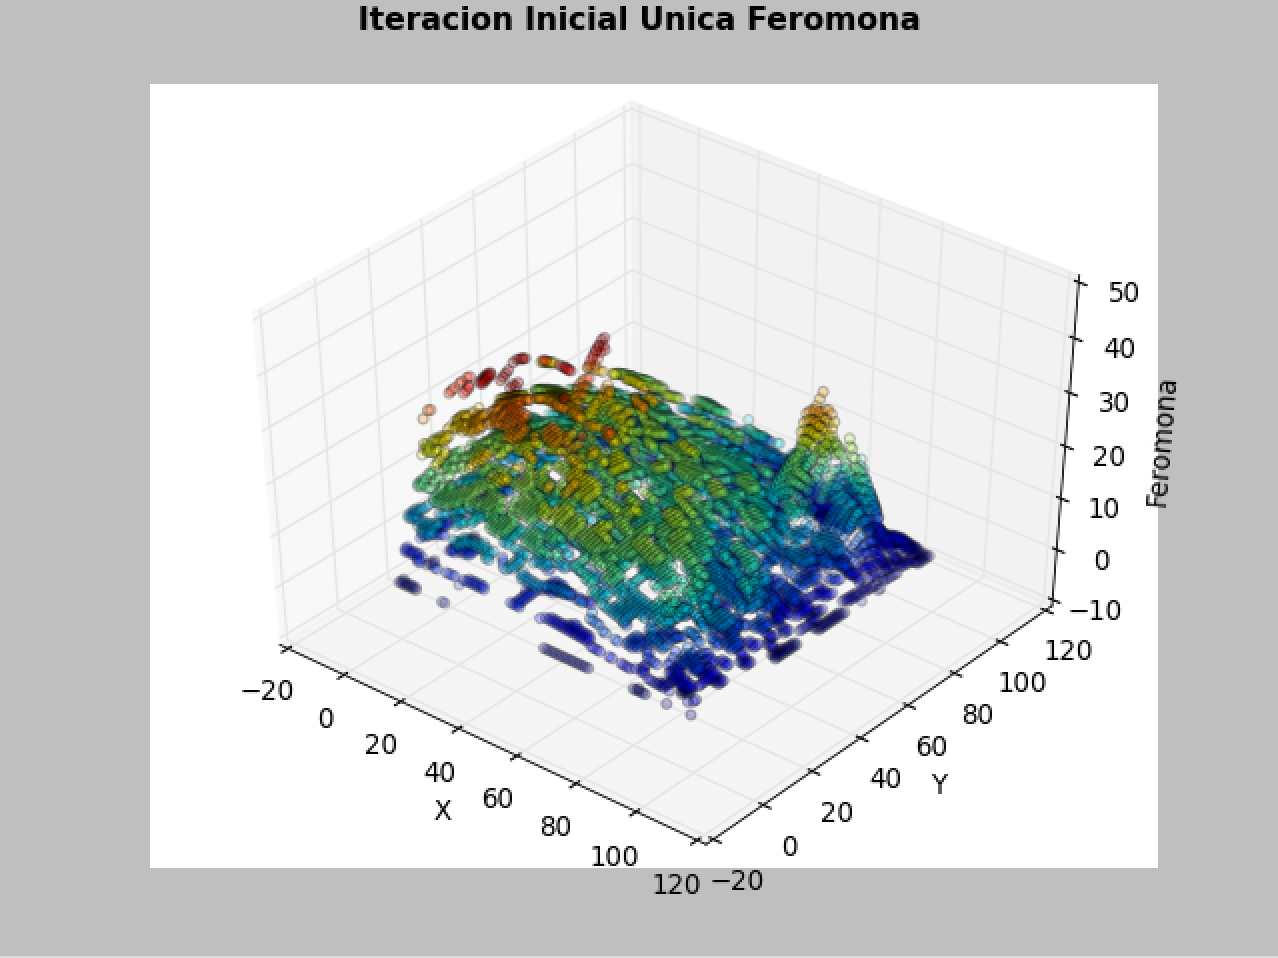
\includegraphics[width=0.49\textwidth]{imagenes/iter-1}
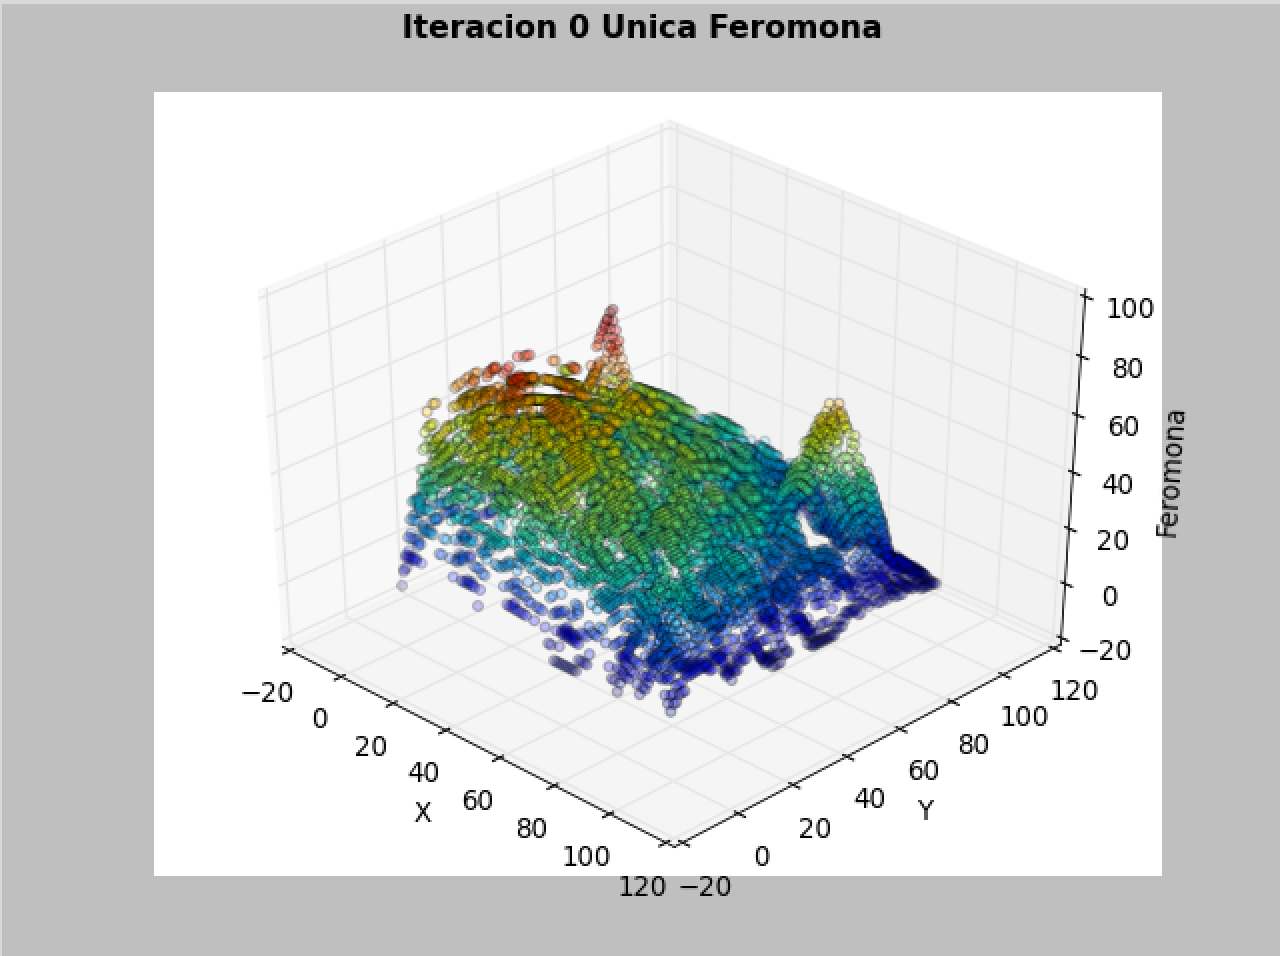
\includegraphics[width=0.49\textwidth]{imagenes/iter0}
\end{center}
\begin{center}
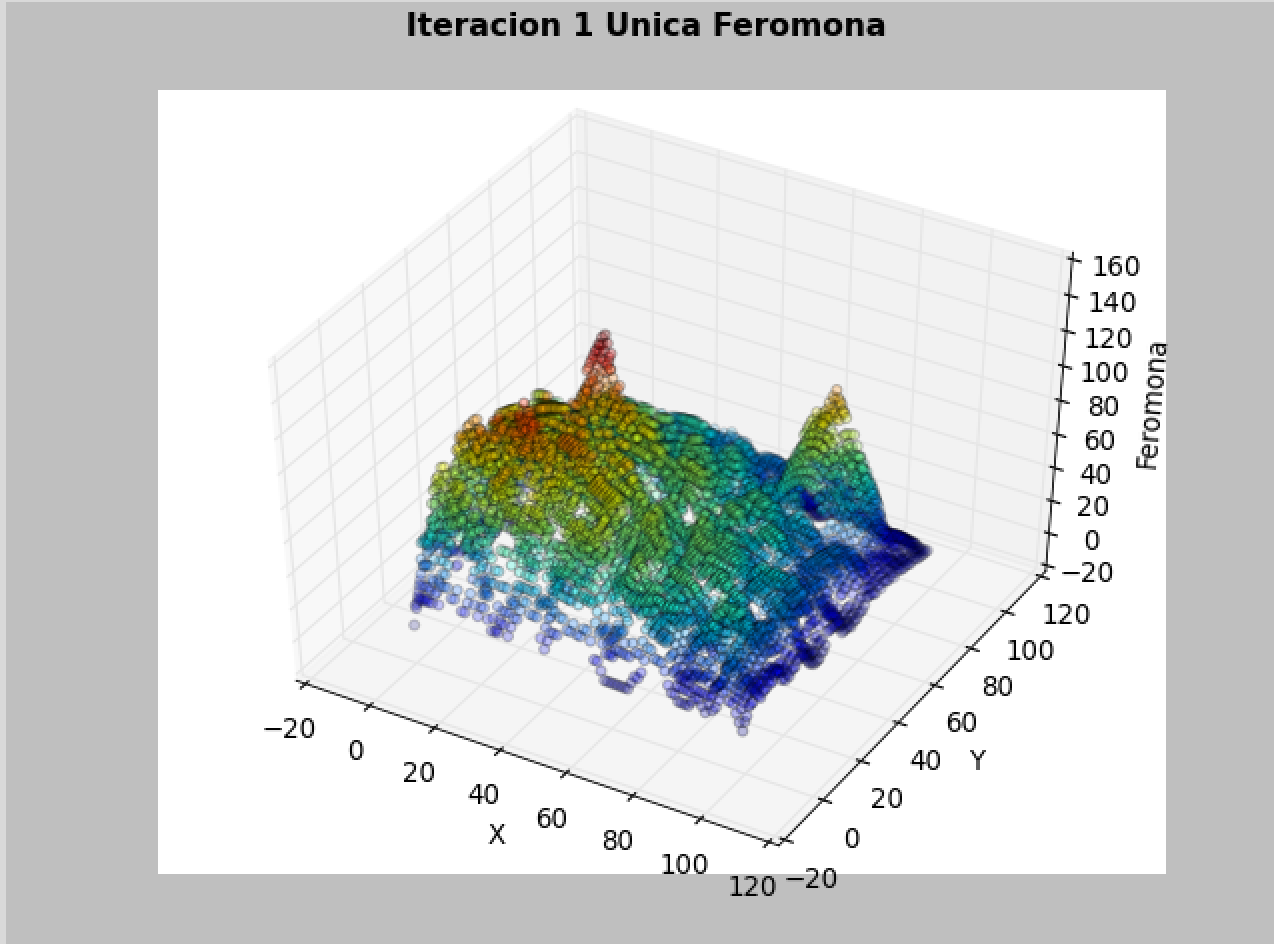
\includegraphics[width=0.49\textwidth]{imagenes/iter1}
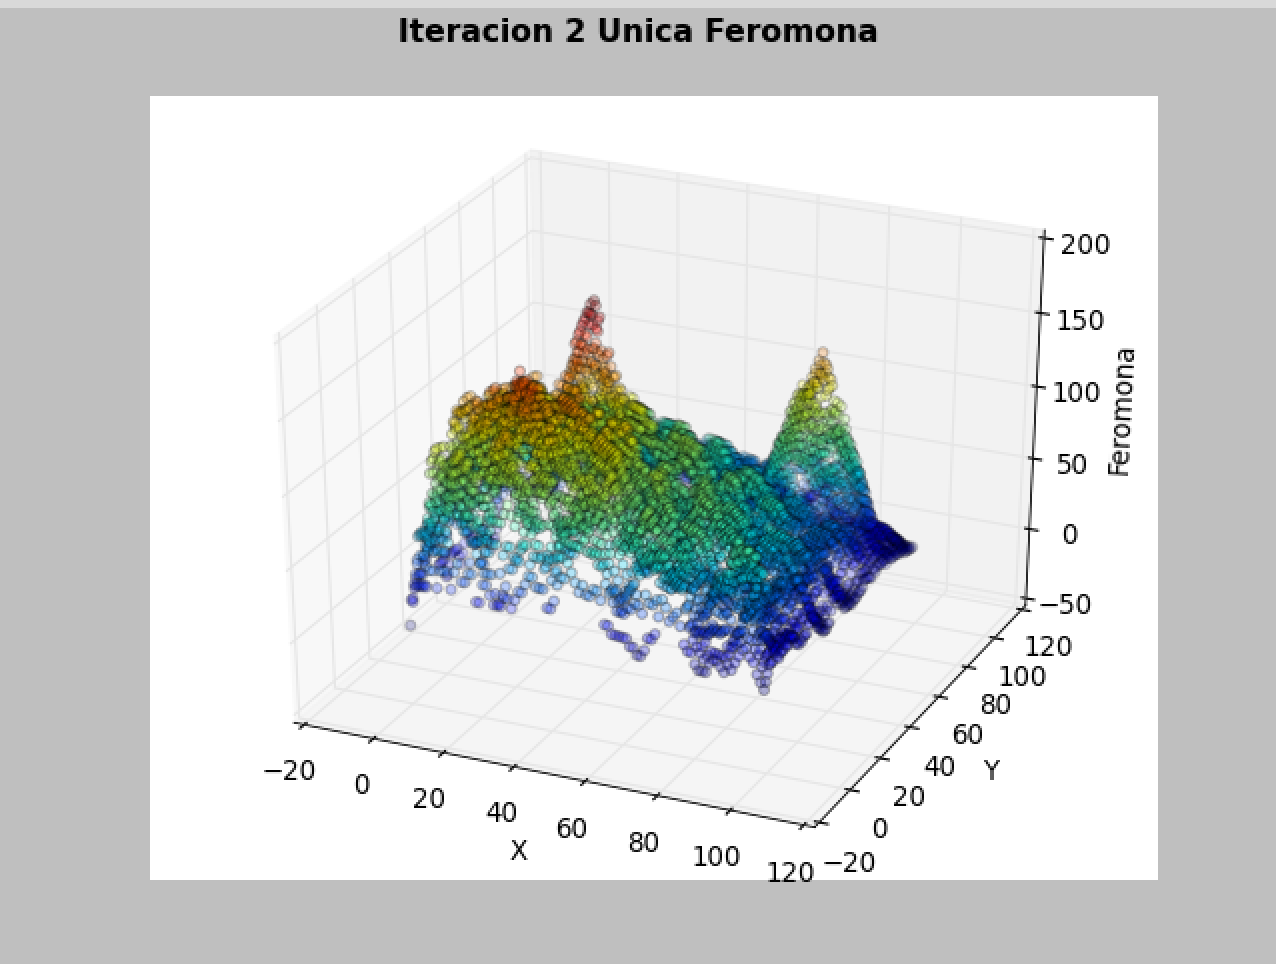
\includegraphics[width=0.49\textwidth]{imagenes/iter2}
\end{center}
\begin{center}
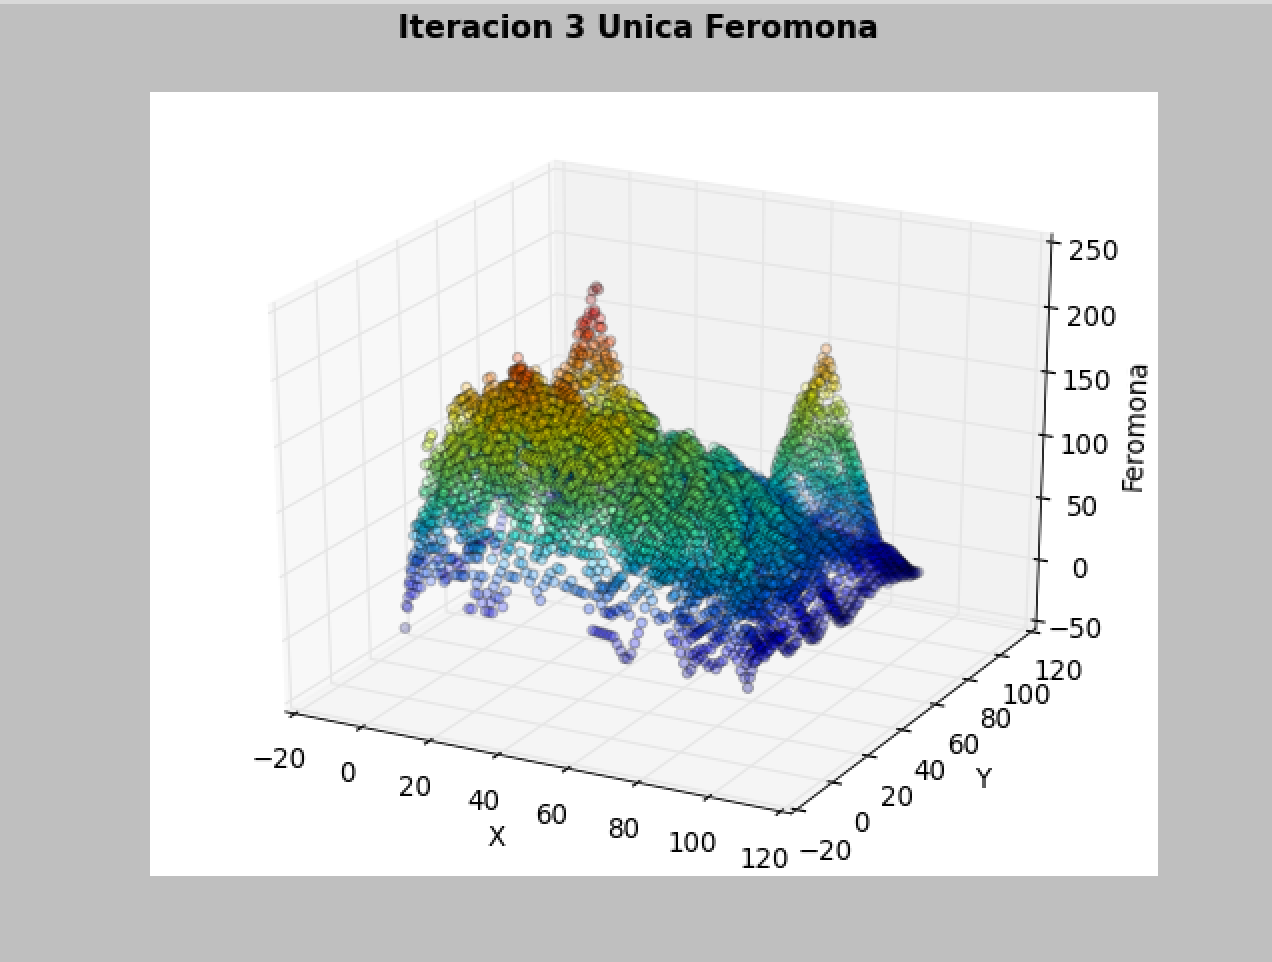
\includegraphics[width=0.49\textwidth]{imagenes/iter3}
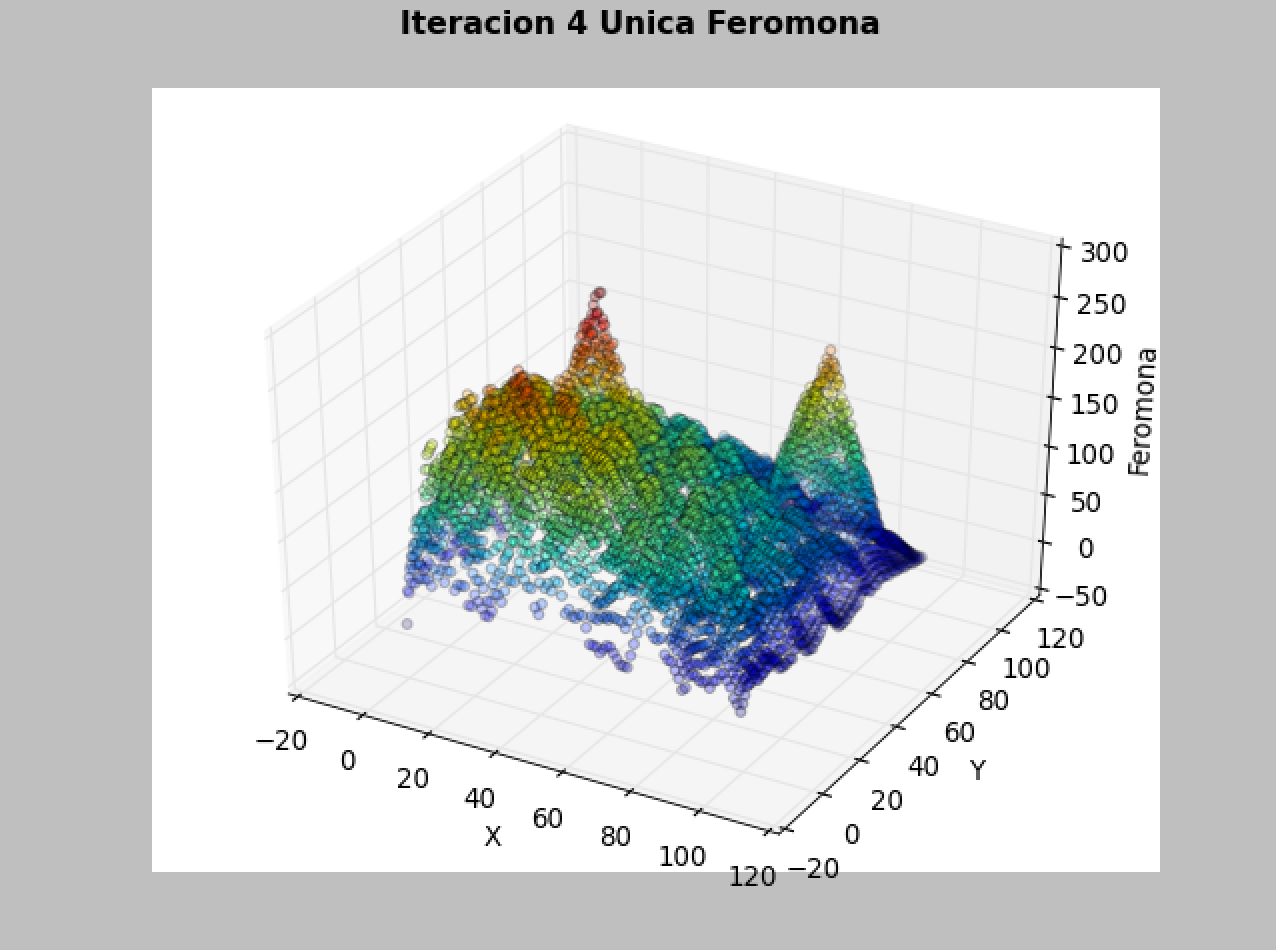
\includegraphics[width=0.49\textwidth]{imagenes/iter4}
\end{center}

\newpage

Veamos a continuaci\'on el mismo ejemplo pero con la versi\'on 2 de colonia de hormigas.

\begin{center}
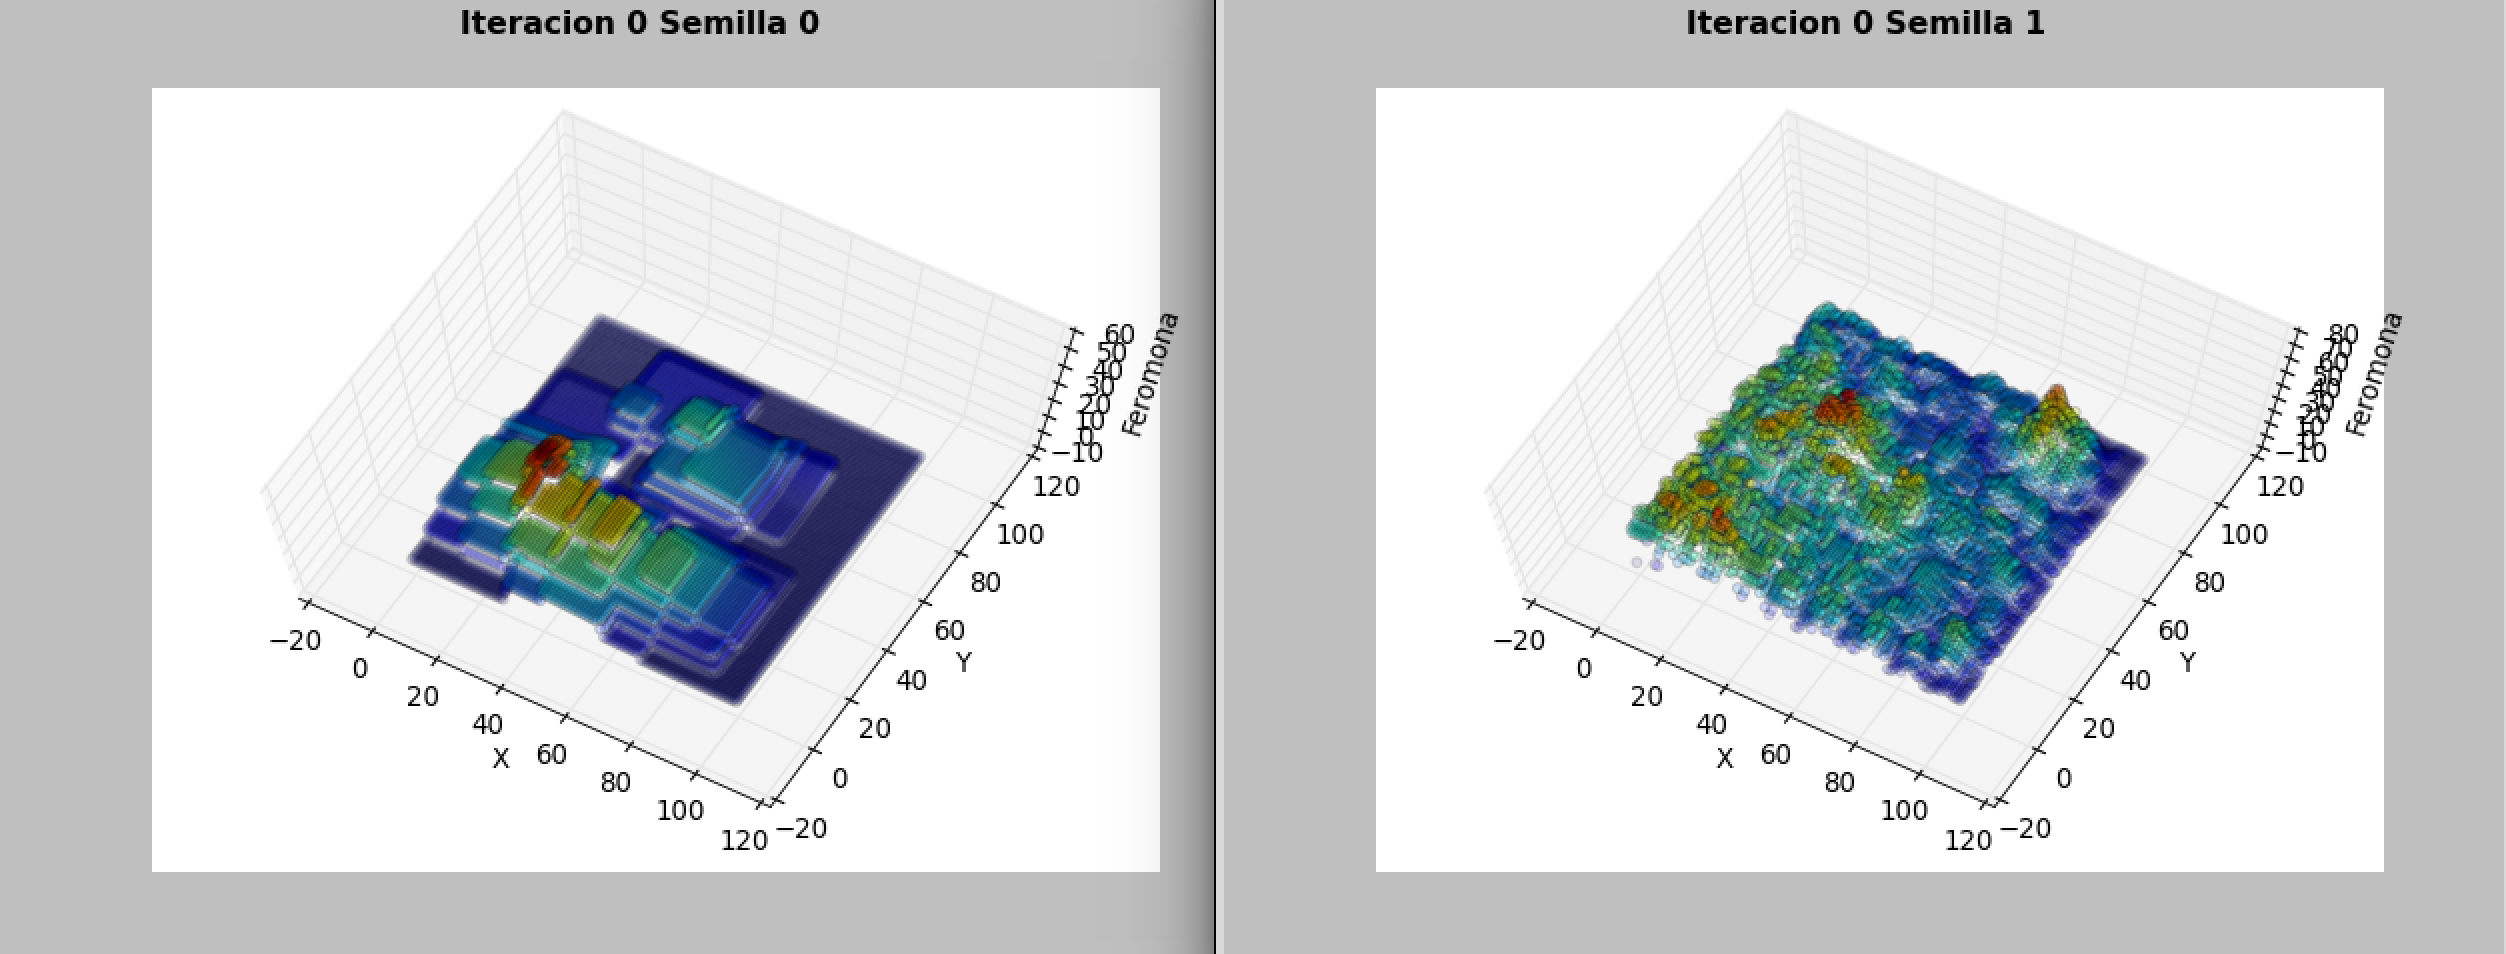
\includegraphics[width=1\textwidth]{imagenes/dobleiter0}
\end{center}
\begin{center}
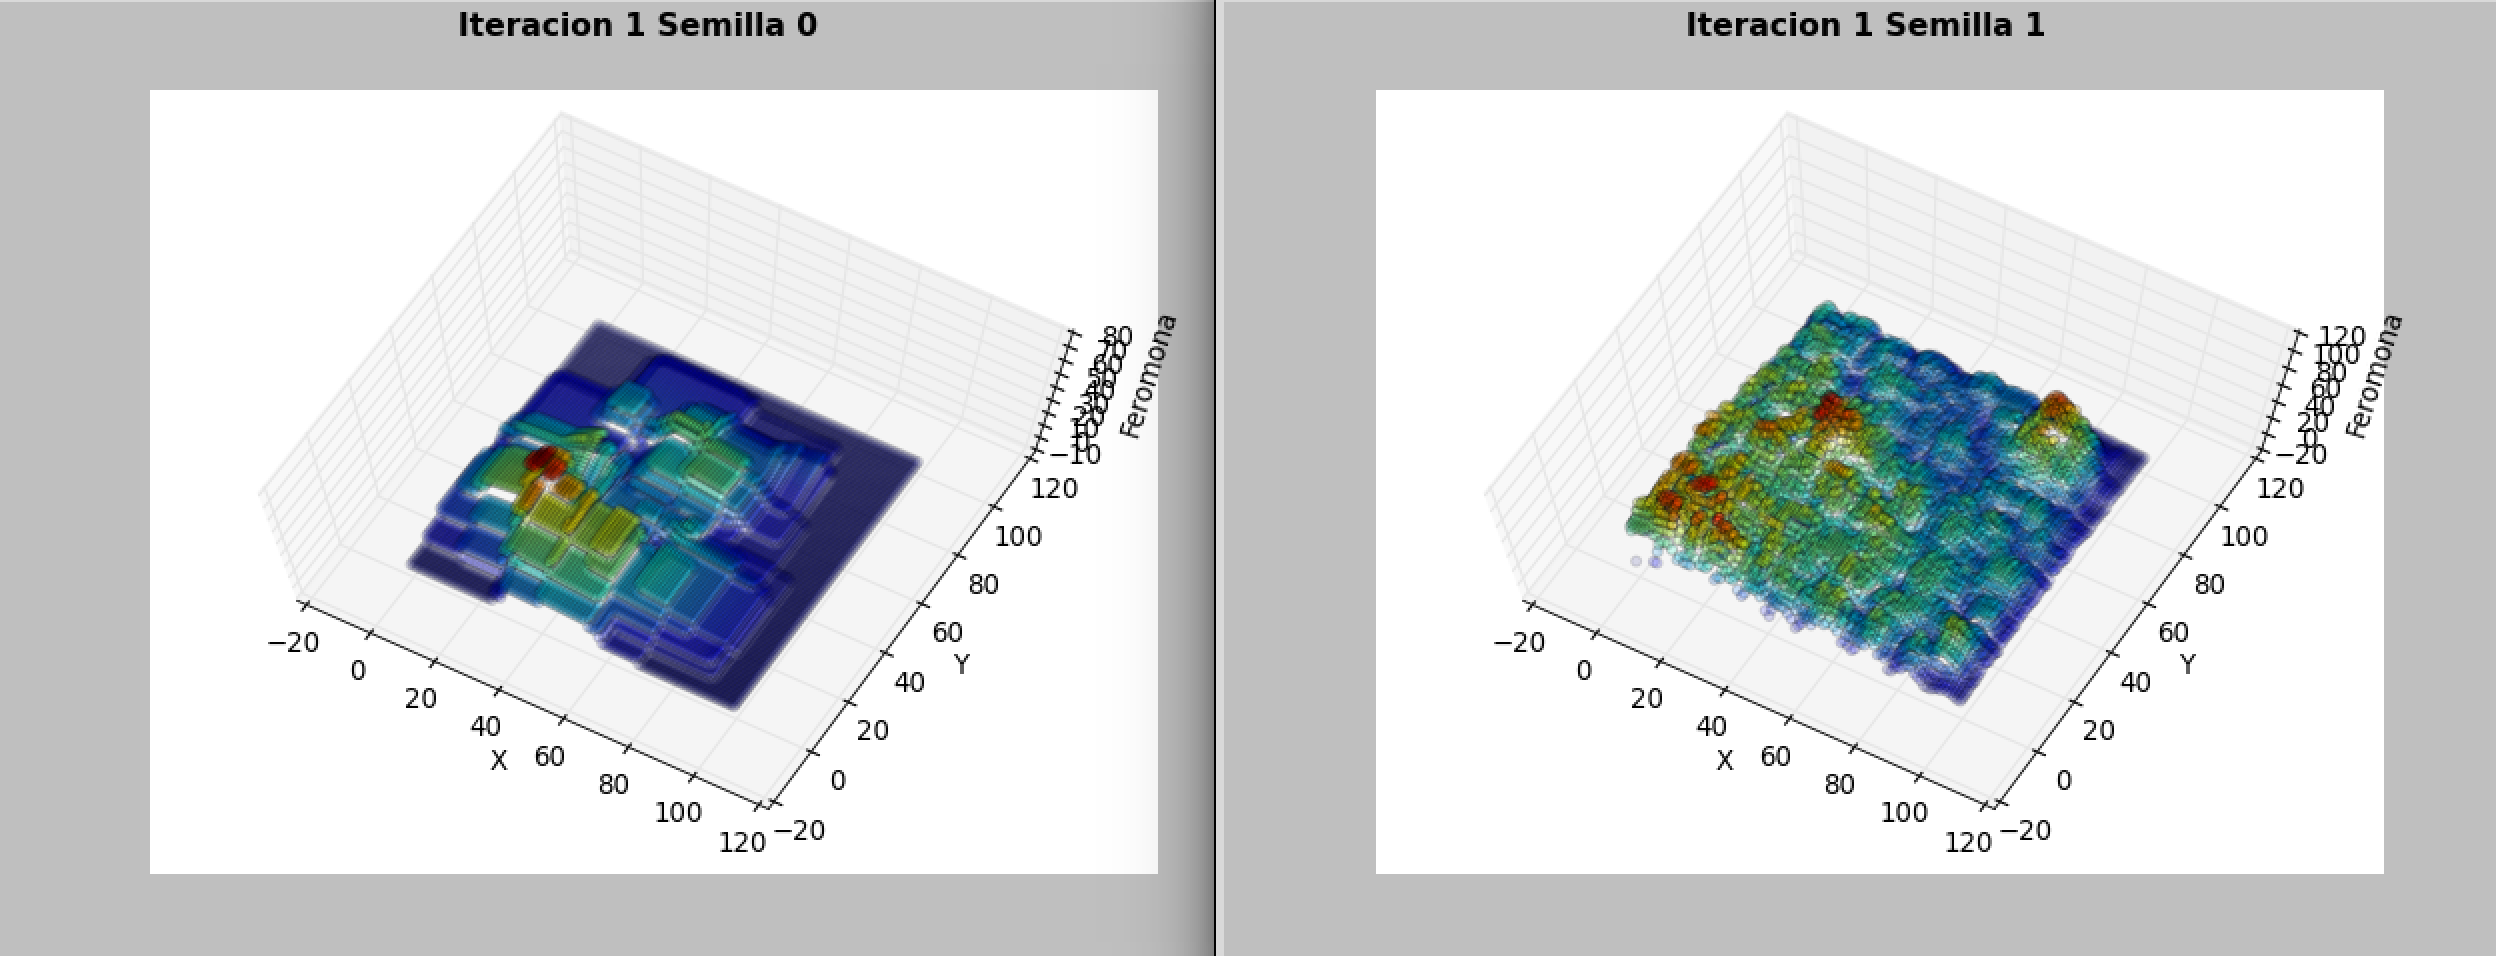
\includegraphics[width=1\textwidth]{imagenes/dobleiter1}
\end{center}
\begin{center}
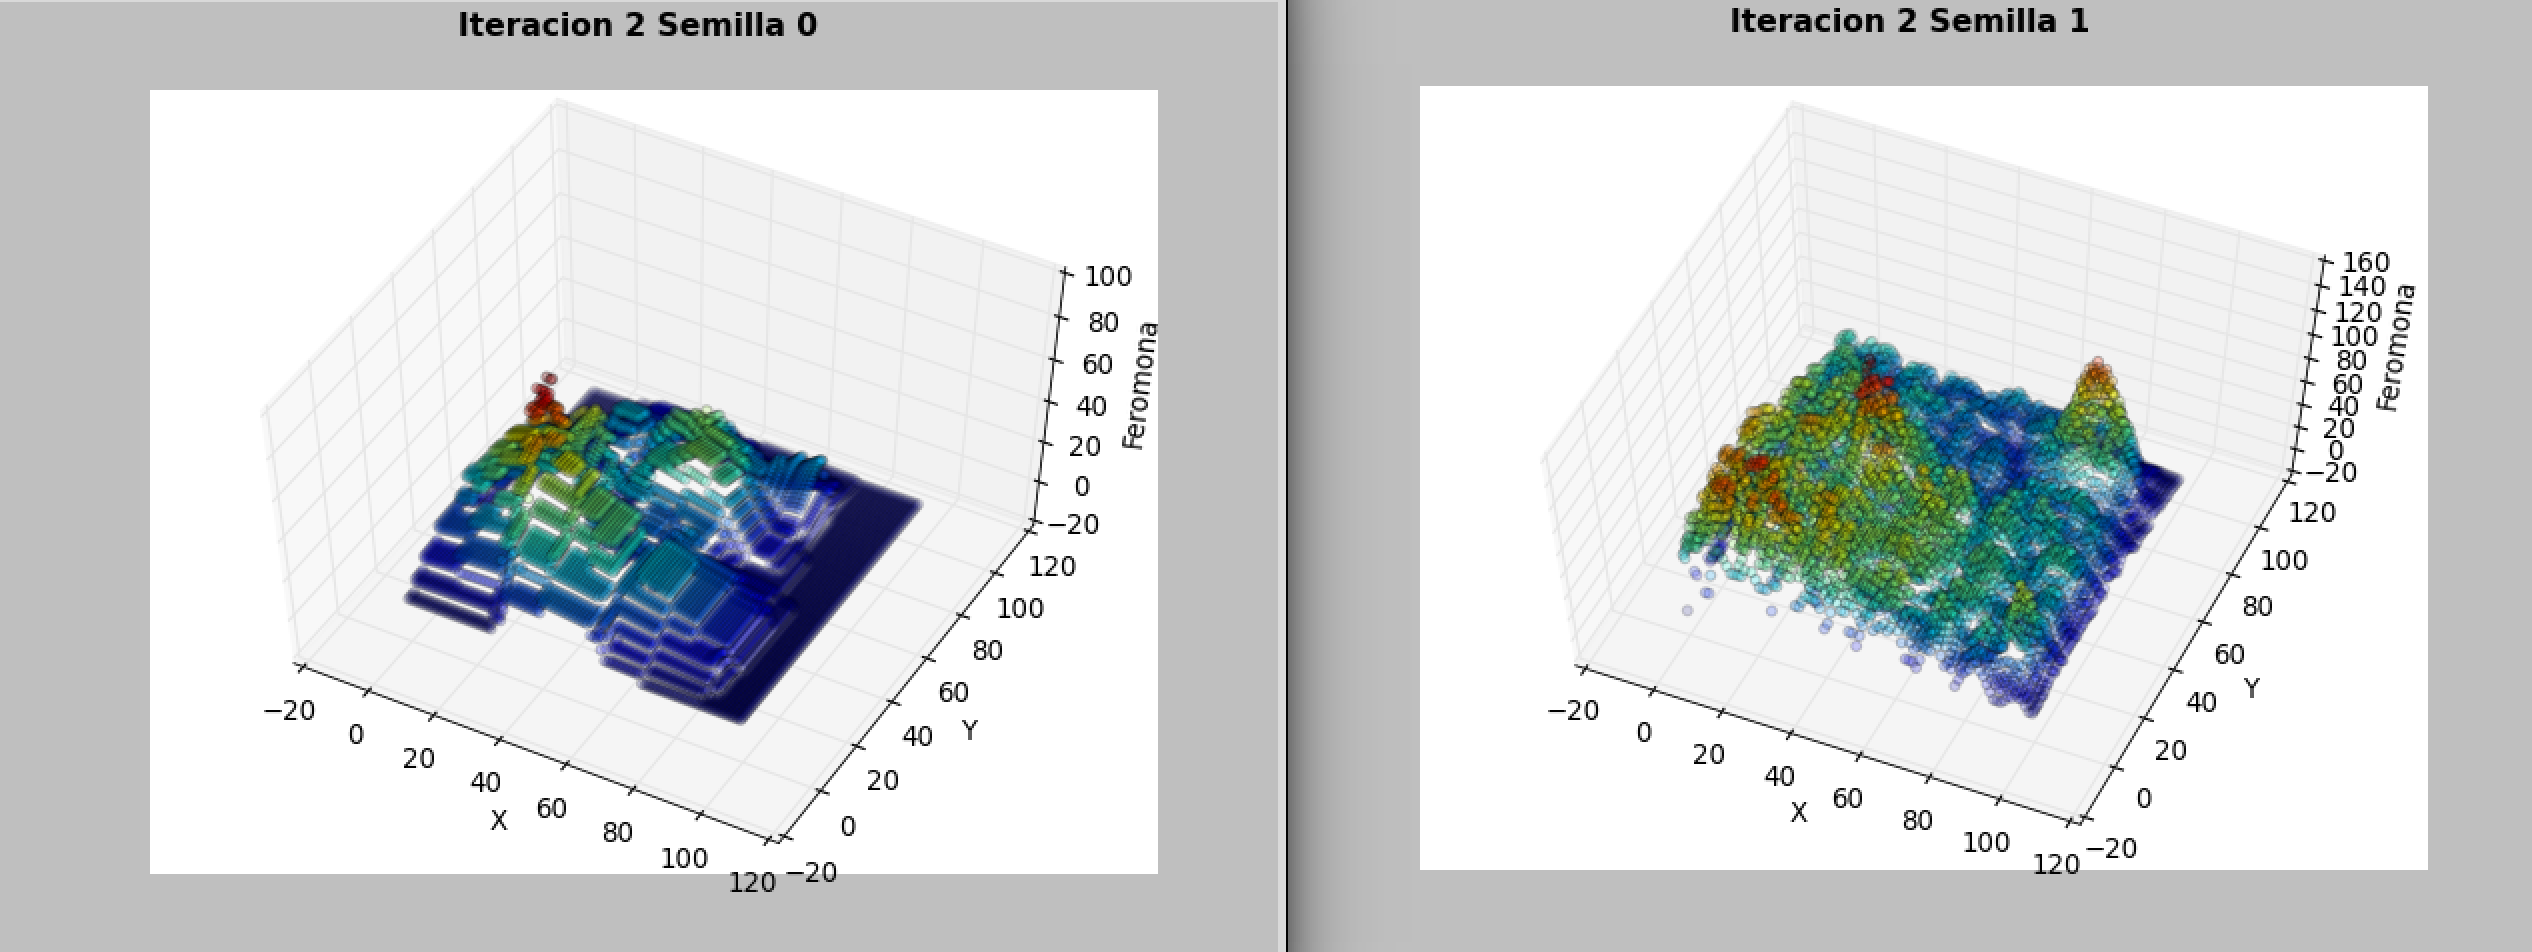
\includegraphics[width=1\textwidth]{imagenes/dobleiter2}
\end{center}
\begin{center}
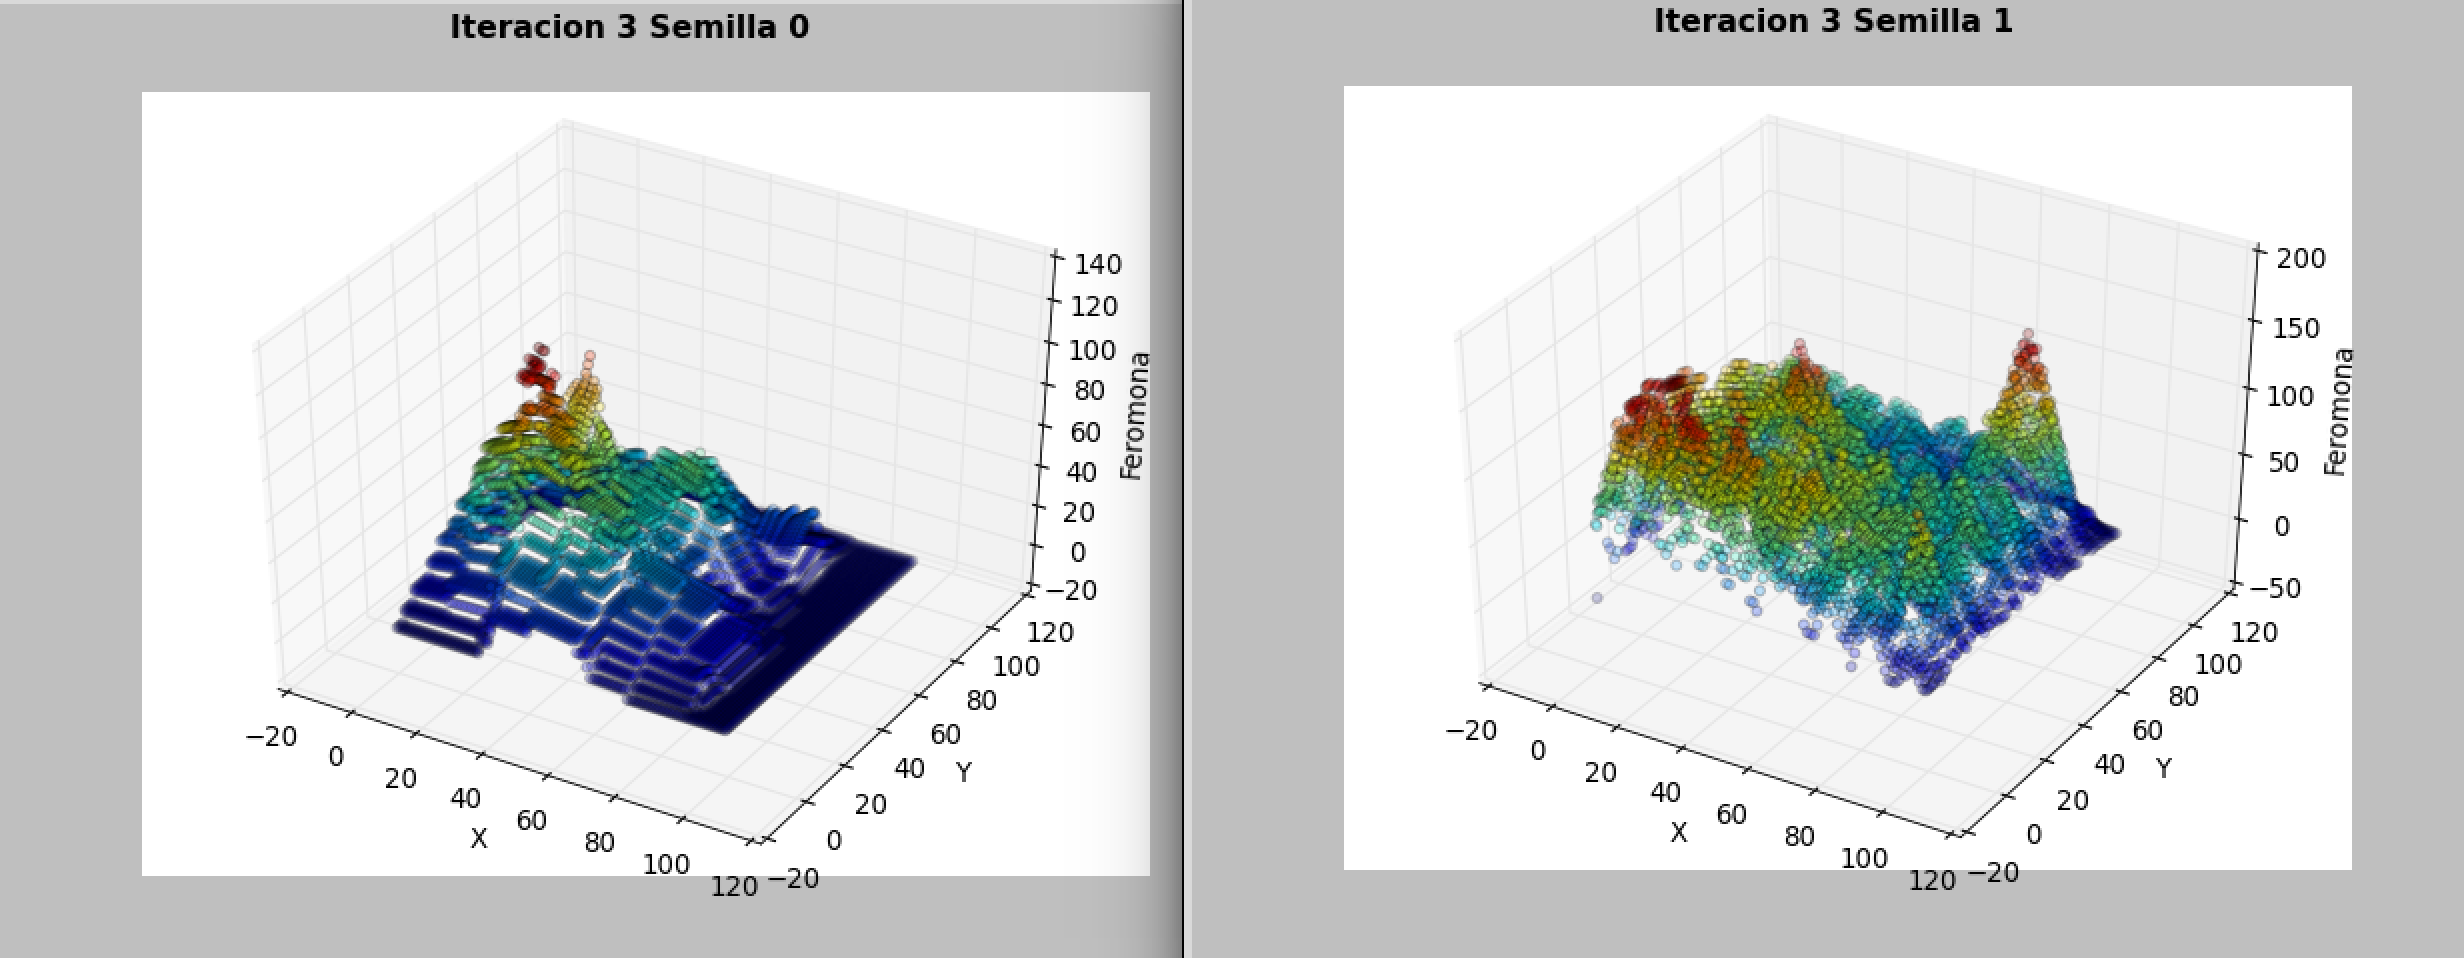
\includegraphics[width=1\textwidth]{imagenes/dobleiter3}
\end{center}

El comportamiento es id\'entico al algoritmo anterior, pero notemos que para cada iteraci\'on tenemos 2 gr\'aficos de feromonas, esto es porque tenemos 2 semillas, y por lo tanto una feromona por semilla.

Si miramos con atenci\'on, podemos notar que en los gr\'aficos de la semilla 0 se notan marcados los pads mas grandes en la funci\'on de feromona, esto es porque la semilla 0 corresponde a los pads grandes. En cambio en la feromona de la semilla 1 es un poco menos uniforme dado que corresponde a una semilla mucho m\'as chica. 	
